%------------------------------------------------------------------------------
% Sam Nazari
% Spring 2016: Manuscript for journal submission
%------------------------------------------------------------------------------
%
% AMS-LaTeX version 2 sample file for journals, based on amsart.cls.
%
\documentclass[reqno,8pt]{amsart}
%     If your article includes graphics, uncomment this command.
\usepackage[final]{graphicx}
\usepackage[text={7in,10in},centering,top=72pt,bottom=54pt,right=54pt,left=54pt]{geometry}
\usepackage{color}
\usepackage{amsmath}
\usepackage{amssymb}
\usepackage[linesnumbered,ruled]{algorithm2e}
\usepackage{amsfonts}
\usepackage{graphicx}
\usepackage{hyperref}
\usepackage{float}
\usepackage{caption}
\usepackage[numbers,sort&compress]{natbib}
\usepackage{tikz}
\usepackage{setspace} % Double spacing
%\doublespacing
\pdfminorversion=4
\usepackage{subcaption}
\hypersetup{
    bookmarks=true,         % show bookmarks bar?
    unicode=false,          % non-Latin characters in Acrobat’s bookmarks
    pdftoolbar=true,        % show Acrobat’s toolbar?
    pdfmenubar=true,        % show Acrobat’s menu?
    pdffitwindow=false,     % window fit to page when opened
    pdfstartview={FitH},    % fits the width of the page to the window
    pdftitle={Network Attack Tolerance Optimization},    % title
    pdfauthor={Sam Nazari},     % author
    pdfsubject={Instrusion Detection},   % subject of the document
    pdfcreator={Sam Nazari},   % creator of the document
    pdfproducer={Sam Nazari}, % producer of the document
    pdfkeywords={Intrusion Detection} {Expander Graph} {Spectral Algorithm}, % list of keywords
    pdfnewwindow=true,      % links in new PDF window
    colorlinks=false,       % false: boxed links; true: colored links
    linkcolor=red,          % color of internal links (change box color with linkbordercolor)
    citecolor=green,        % color of links to bibliography
    filecolor=magenta,      % color of file links
    urlcolor=cyan           % color of external links
}

\newtheorem{theorem}{Theorem}
\newtheorem{corollary}{Corollary}
\newtheorem{lemma}{Lemma}
\newtheorem{prop}{Proposition}
\theoremstyle{definition}
\newtheorem{definition}{Definition}
\newtheorem{example}[theorem]{Example}
\newtheorem{xca}[theorem]{Exercise}
\newtheorem{app}{Application}
\newtheorem{ass}{Assumption}
\newtheorem{cond}{Condition}
\newtheorem{problem}{Problem}

\theoremstyle{remark}
\newtheorem{remark}{Remark}

\numberwithin{equation}{section}

%    Absolute value notation
\newcommand{\abs}[1]{\lvert#1\rvert}

%    Circled numbers
\newcommand*\circled[1]{\tikz[baseline=(char.base)]{
            \node[shape=circle,draw,inner sep=2pt] (char) {#1};}}
            
%    Blank box placeholder for figures (to avoid requiring any
%    particular graphics capabilities for printing this document).
\newcommand{\blankbox}[2]{%
  \parbox{\columnwidth}{\centering
%    Set fboxsep to 0 so that the actual size of the box will match the
%    given measurements more closely.
    \setlength{\fboxsep}{0pt}%
    \fbox{\raisebox{0pt}[#2]{\hspace{#1}}}%
  }%
}

\sloppy
\definecolor{lightgray}{gray}{0.5}
\setlength{\parindent}{0pt}

\def\X{b}
\def\tX{\tilde{b}}
\def\mX{B}
\def\tmX{\tilde{B}}
\def\bone{{\bf 1}}
\def\bzero{{\bf 0}}
\def\bx{{\bf x}}
\def\by{{\bf y}}
\def\bz{{\bf z}}
\def\bof{{\bf f}}
\def\N{\mathbb{N}}
\def\Z{\mathbb{Z}}
\def\Q{\mathbb{Q}}
\def\R{\mathbb{R}}
\def\C{\mathbb{C}}
\def\mP{\mathbb{P}}
\def\mE{\mathbb{E}}
\def\mI{\mathbb{I}}
\def\cN{\mathcal{N}}
\def\cV{\mathcal{V}}
\def\cE{\mathcal{E}}
\def\cC{\mathcal{C}}
\def\cT{\mathcal{T}}
\def\cS{\mathcal{S}}
\def\cP{\mathcal{P}}
\def\cB{\mathcal{B}}
\def\cVGD{\mathcal{V}_{G_d}}
\def\cEGD{\mathcal{E}_{G_d}}
\def\cVHD{\mathcal{V}_{H_d}}
\def\cEHD{\mathcal{E}_{H_d}}
\def\eps{\epsilon}
\def\reff{\textup{Reff}}
\def\deg{\textup{deg}}
\def\GD{G_d=(\cVGD,\cEGD)}
\def\HD{H_d=(\cVHD,\cEHD)}
\newcommand{\etal}{\textit{et al}. }
\newcommand{\ie}{\textit{i}.\textit{e}., }
\newcommand{\eg}{\textit{e}.\textit{g}. }

\DeclareMathOperator*{\argmax}{\arg\!\max}

\begin{document}
\pagenumbering{gobble}
\title{Design of Attack Tolerant Detection Topologies For Distributed Systems}
%\title{On Resilience in Network Topology Design}
%\title{Resilient Network Topology Design}
%\title{Optimal Network Topology Resilience Design}
%\title{Network Topology Attack Tolerance Optimization}
% \title{Maximum Attack Tolerance by Optimal Spectral Expansion}
% \title{Maximum Attack Tolerance by Spectral Expansion Optimization}

%    Information for first author
\author{Sam Nazari, Bahram Shafai \& Amirreza Oghbaee}
%    Address of record for the research reported here
%\address{Northeastern University}
%    Current address
%\curraddr{Department of Mathematics and Statistics,
%Case Western Reserve University, Cleveland, Ohio 43403}
%\email{nazari@ece.neu.edu}
%    \thanks will become a 1st page footnote.
%\thanks{The first author was supported in part by NSF Grant \#000000.}

%    Information for second author
%\author{Author Two}
%\address{Mathematical Research Section, School of Mathematical Sciences,
%Australian National University, Canberra ACT 2601, Australia}
%\email{two@maths.univ.edu.au}
%\thanks{Support information for the second author.}

%    General info
%\subjclass[2000]{Primary 54C40, 14E20; Secondary 46E25, 20C20}

%\date{07-February-2016}

%\dedicatory{This paper is dedicated to our advisors.}

%\keywords{Spectral Expansion, Expanders, Intruder Detection, Robust Graph Topologies.}

\begin{abstract}
Let $G=(\cV_G,\cE_G)$ be a network consisting of $n$ agents such that $k < n$ of the agents are malicious agents and let $H=(\cV_H,\cE_H)$ be a subgraph within $G$ consisting of agents equipped with detection filters to identify intrusions by malicious agents. Assume that $G$ is also under attack from an external adversary whose goal is to disconnect the largest set of vertices in $H$ by sabotaging $\epsilon$ fraction of its edge set, leaving the detection filters unable to sense intrusions from malicious agents. This paper establishes the algebraic and combinatorial conditions under which $H$ is maximally robust to attacks from external adversaries.  It is shown that the combinatorial problem of extracting a robust topology for $H$ can be formulated as an optimization problem involving the Laplacian spectrum of $G$. An algorithm is given to recover the desired topology with the property that after an $\epsilon$ fraction of the edges are adversarially removed, the network still maintains a connected component that spans at least $(1-\frac{\epsilon}{2\phi})$ fraction of the vertices, with $\phi$ denoting the conductance of $G$. For the class of similar graphs that are cospectral, we also relate the algebraic connectivity to the third moment of the adjacency matrix of $G$, paving the way for an alternative means of obtaining $H$ instead of the spectral approach. 
\end{abstract}

\maketitle

% %-----------Introduction--------------
\section{Introduction}
Modern society relies on critical infrastructures that are fundamentally networked \cite{teixeira_secure_2015-1,Pas2015}. Such complex infrastructures comprise of smaller subsystems, referred to as agents, that are interconnected by local information pathways.  Exemplary infrastructures include information bearing networks, financial transaction networks, energy production networks, health care networks, gas distribution networks, water distribution networks, transportation networks, and telecommunication networks \cite{guo_optimal_2016,pasqualetti_time-varying_2017,leong_network_2016,leong_network_2014}. A collection of such agents whose interactions are constrained to involve only a local set of neighboring agents is known as a distributed system.    

% Pas2013 (Attack detection and identification in cyber physical systems) 
% Pas2012 (Consensus computation in unreliable networks: a system theoretic approach)
% PasPhd2012
% Pas2007 (distributed intrusion detection for secure consensus computations)
% Pas2010 (Identifying cyber attacks via local model information)

\medskip

The design of distributed systems is inherently a multidisciplinary endeavor \cite{teixeira_PhD,PasPhd2012, cardenas_research_2008}.  Due to recent high profile incidents (see \eg \cite{fichtner_cybersecurity_2016,WHNYT2015,lipton_perfect_2016,gorman_electricity_2009}), major emphasis and attention is now being directed at developing rigorous analytic tools to evaluate the vulnerabilities that can lead to unexpected service disruptions in critical infrastructures involving networked control systems (NCS) and Cyber-Physical Systems (CPS) \cite{teixeira_secure_2015,pasqualetti_attack_2013,teixeira_attack_2012,pasqualetti_design_2015,sou_detection_2012,pasqualetti_consensus_2012,teixeira_strategic_2015,sadamoto_weak_2016,park_when_2016,guo_worst-case_2016,Nazari2016}. To meet these challenges, investigators have proposed sophisticated approaches based on systems theory in order to model attack scenarios of malicious agents, see \eg \cite{teixeira_secure_2015,teixeira_secure_2015-1,tarraf_quantifying_2013,teixeira_attack_2012,pasqualetti_control-theoretic_2015,teixeira_PhD,PasPhd2012}. 

\medskip

Moreover, the role of agents in a distributed system has also been under consideration by investigators. For example, the authors of \cite{shames_agents_2012} view each agent as an entity that may potentially ``cause a system wide failure'', or alternatively, ``improve the performance or even enable us to achieve an objective.'' The authors then reason that this view of the role of agents in a distributed system justifies the need for ``monitoring agents in a network to detect if they are misbehaving or not.''  The authors consequently propose a ``distributed method in which each agent monitors its neighbors for any signs of misbehaviors.''  The distributed method referred to in \cite{shames_agents_2012} is strongly rooted in systems theory and is in part an extension of robust observer theory to the distributed setting (see \eg \cite{teixeira_distributed_2014,shames_distributed_2011,teixeira_networked_2010}.)  

\medskip

The sound approach proposed by investigators relying on observer theory raises a related question: what are the objectives that the designer must keep in mind when selecting the subset of monitoring agents? Relatedly, the designer may wish to quantify the robustness of the topology in the network under structural perturbations. With respect to this critical question, investigators have considered various aspects related to the topology of the graphs that model the interactions within distributed systems \cite{leong_network_2016,Akoglu2015,Dek2004,Summers2015,weimer_distributed_2012,lucchese_distributed_2014,besselink_string_2016,Dinh2015,Dinh2012,Feng2015,Kis2013,rieger_resilient_2012,Van2013,Lamp1982,Bien1989}. One major approach involves modeling network vulnerabilities as additive stochastic disturbances in the consensus dynamics of a given network. To quantify the variation about the nominal consensus solution, measures based on the coherence of the underlying network have been proposed. Under this setting, the $\mathcal{H}_2$ norm of the underlying system associated with the network has recently emerged as a meaningful measure of network robustness \cite{Bam2012,Pat2014,Teg2015,Lin2014}.

\medskip

Separately, investigators have also proposed various notions of \textit{resilience} in order to quantify tolerance to disruptions in a network \cite{rieger_resilient_2009,sadamoto_weak_2016, biswas_resilient_2012,rieger_resilient_2012,garcia_resilient_2014,zeng_resilient_2014,Basar2012a,Basar2013,Wente2014,Basar2011}. More intuitively, resilience is sometimes referred to as the \textit{error} or \textit{attack tolerance}\cite{Chan2016} of an interconnected or distributed system. Roughly speaking, a resilient system is one that maintains an accepted level of operational normalcy in response to disturbances, including faults within the agents, in between the communications pathways of agents or any combination of the above due to an attack by a malicious entity \cite{rieger_resilient_2009}. When the system under consideration is a distributed system that can be modeled by a graph, this definition may be adapted in a more quantitative way by defining a graph to be resilient if it is capable of retaining its structural and connectivity properties after losing $\epsilon$ portion of its edge set. In \cite{Banerjee2009,Banerjee2011} the authors consider the problem of distributed fault-tolerance and propose algorithms and a framework to accommodate multiple fault regions under the constraint that each fault region is highly localized. In \cite{Pinar2010} the authors consider the problem of finding a small set of lines or edges whose loss or removal can cause a severe blackout in a power network setting and focus on identifying the links that can cause major blackouts. In \cite{Basar2012b}, the problem of forming consensus under the presence of an intelligent adversary whose objective is to slow down the convergence rate of the network to the global average is considered. 

\medskip

Beyond the notions of resilience and robustness, investigators continued to expand the horizons of the field by considering problems pertaining to identification of useful structures within distributed systems. For example, the authors of \cite{Akoglu2015} devise an algorithm to extract the maximum clique from within a network. 
% In practice, however, it can be shown that the maximum clique subgraph has minimal stability margins with respect to perturbations in the overall graph\cite{Gharan2015}. Furthermore, there is no extension of the maximum clique problem for weighted graphs, which limits their applicability in modeling many real world distributed systems. Finally, cliques can easily be targeted by a malicious adversary who deletes a fraction of the edges of the network uniformly at random. 
Similarly, in \cite{Van2013}, the authors consider the problem of finding the critical region of a distributed system which would lead to the highest network disruption if it were disconnected from the rest of the network. In \cite{Shafi2010}, the authors consider the problem of designing an interconnection topology such that the gap between the largest and smallest Laplacian eigenvalues is optimized. Their SDP formulation reassigns the edge and vertex weights in such a manner so that the spectral gap between the largest and smallest Laplacian eigenvalue is minimized. In \cite{dahan_security_2016}, the authors consider a two-player strategic game for network routing under link disruptions. Player 1 is the defender and routes flow through a network to maximize her value of effective flow while facing transportation costs. Player 2 is the attacker who aims to disrupt one or more links to maximize her value of lost flow but also faces cost of disrupting links.

\medskip

The present paper is motivated by the need to develop rigorous tools for constructing resilient intrusion detection topologies for use in critical infrastructures. To that end, section \ref{sec:background} sets the background for the problem considered and summarizes our results. Section \ref{sec:Prelim} reviews the fundamentals of spectral graph theory and provides a new result (Theorem \ref{thrm:algTriangle}) relating the graph expansion to the third moment of the graph adjacency matrix. %Further, our previous models for malicious agents in a distributed setting as well as the internal monitoring agents are reviewed. 
Section \ref{sec:problemFormulationSpecRecovery} formulates the problem addressed in this paper and states the main results along with spectral algorithms to recover the optimal topology. Finally, an illustrative example is provided in Section \ref{sec:Example} and we conclude in Section \ref{sec:sec5}.   

%-----------Background--------------
% \begin{figure}
%     \centering
%     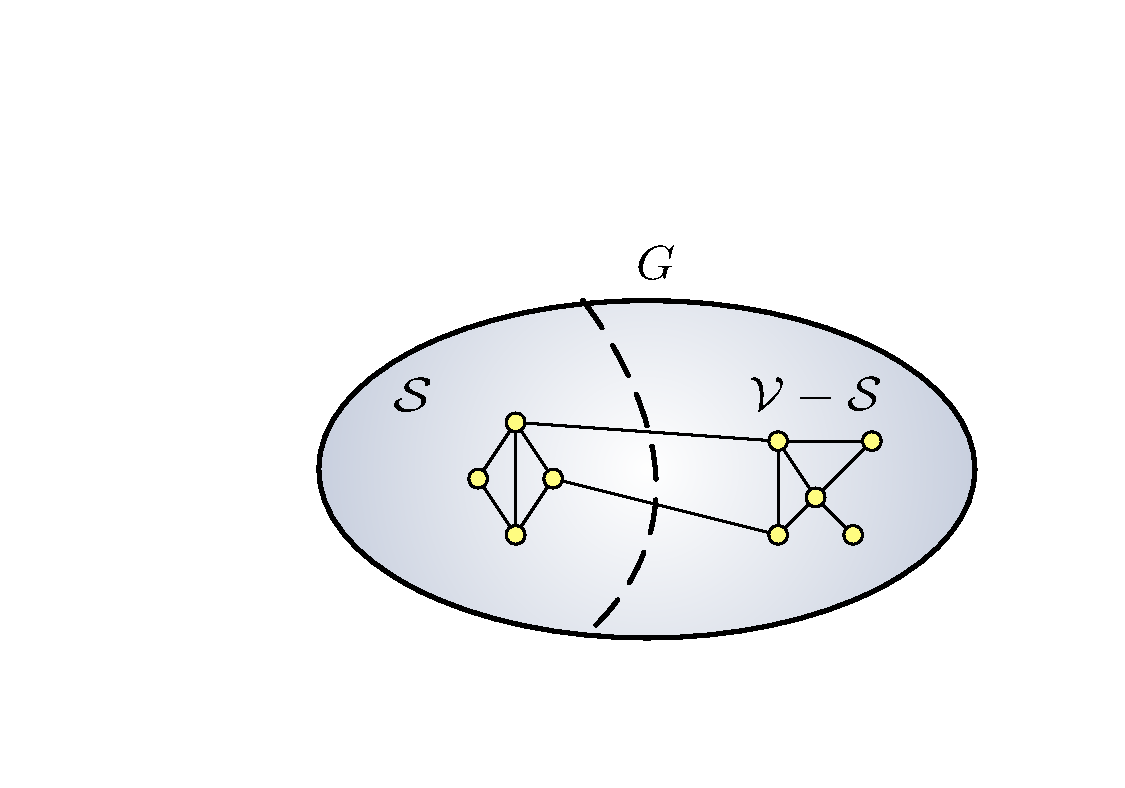
\includegraphics[scale=0.25]{GraphCut}
%     \caption{A graph cut illustrated conceptually. The cut is shown in dashed lines. }
%     \label{fig:graphCut}
% \end{figure}
\section{Background} \label{sec:background}
Let $G = (\cV_G, \cE_G)$ be a network over $n$ agents wherein $k < n$ intruders are known to be present. It has recently been shown that any subset of the remaining $n-k$ agents can be tasked with monitoring the network in search of the intruder by endowing them with detection filters \cite{Nazari2016}. Denote the network of monitoring agents by $H=(\cV_H,\cE_H)$. %When $\cV_H \subset \cV_G$ and $\cE_H \subset \cE_G$, then $H$ is a subgraph in $G$, denoted by $H \subset G$.  
We assume that an external adversary intends to mount a catastrophic attack on $H$. Such an attack could be the caused by a natural disaster or a jamming signal designed to disrupt inter force communications under electronic warfare scenarios \cite{Feng2015,Naz05}. Regardless of the actual underlying cause, the result of the external attack is that the network of monitoring agents will be disrupted, leading to  degradation of intrusion detection capabilities by the agents in $H$. 

\medskip

We model external attacks as sparse cuts in $G$.  Graph topologies that admit sparse cuts are considered to be  prime targets for an adversarial attack. This is because the adversary can accomplish its goal of disconnecting the graph by incurring minimum cost, \ie cutting the minimum number of edges. In contrast, the graph topology that offers the most resilience to cuts is the the complete graph. Complete graphs are resilient because the number of edges connecting one subset of verticies to another subset of verticies is maximized. Disconnecting a larger set of edges requires more energy and resources for an adversary. In the jamming scenario alluded to in \cite{Feng2015,Naz05}, this implies that the adversary must transmit at higher power levels, increasing the risk of interception.

\medskip

It is well known that expander graphs are optimal approximations of complete graphs \cite{Lub1994,Lub2012,Lub1988,Wig2006}. It can be shown that the desirable connectivity  properties of complete graphs are preserved by their expander approximations. In particular, it has been shown that the eigenvalues of the Laplacian matrix associated with a $d$-regular expander are the eigenvalues of its corresponding complete graph scaled by $d/n$. Similar relationships have been established with respect to graph cuts, notably that the size of any cut in an expander is equal to $d/n$ fraction of the same cut in a complete graph over the same vertices \cite{Gharan2015}.    

%\medskip
% This paper endeavors to establish the conditions under which a network of monitoring agents, $H$, will possess a topology that is maximally resilient to external attacks. 
% \begin{figure}
%     \centering
%     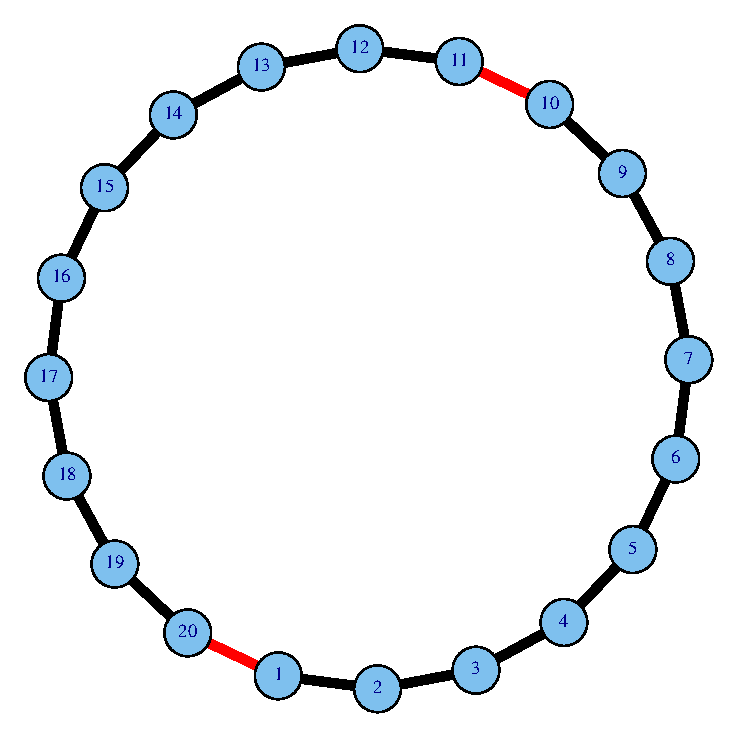
\includegraphics[scale=0.2]{ringGraph.eps}
%     \caption{A ring graph with $n=20$. If this graph is cut at the edges that are colored red, then $n/2$ vertices of the graph will be disconnected. Since a large fraction of graph can be separated with only two cuts, we say that this graph does not have ``good expansion''.}
%     \label{fig:ringGraph}
% \end{figure}

\medskip
In section \ref{sec:problemFormulationSpecRecovery} we show that when $H$ meets special properties then a connected component of size at least $(1-\epsilon/2\phi)$ will remain  after an attack on $\epsilon$ fraction of its edges. The quantity $\phi$ is known as the graph conductance, an important graph invariant that we define precisely in section \ref{sec:Prelim}. The main result, reported as Theorem \ref{thrm:existenceOfH}, establishes the existence of a subgraph within $G$ that consists of at least $\frac{3}{8} \delta n$ monitoring agents that possesses a topology whose spectral expansion (algebraic connectivity) is at least $\frac{\lambda^2\delta^2}{32d log^2 \delta}$. In order to exploit this desirable property, an algorithm is provided to recover the hidden expander from within $G$ (Algorithm \ref{alg:alg2}.) The algorithm depends of two design parameters: one parameter, $\delta$, specifies the size of the desired network of monitoring agents and the other parameter, $\gamma$, specifies a lower bound on the spectral expansion of the resulting network. 
% \medskip

% The next result, reported as Theorem \ref{thrm:ramanujanAgents}, provides a combinatorial construction for $H$ with desirable algebraic properties. For example, given a vertex (monitoring agent) $u$, Theorem \ref{thrm:ramanujanAgents} gives the three adjacent verticies (monitoring agents) that $u$ must be connected to in order to obtain the maximally resilient monitoring agent topology $H$, measured in terms of the spectral expansion $\lambda_2 (\cV_H)$. We refer to the agents in this setting as Ramanujan agents since their resulting topology leads to a Ramanujan expander graph. 

% \medskip

% Theorem \ref{thrm:ramanujanAgents} assumes that $|\cV_H|$ is a prime number, an assumption that may not always be possible to meet in the real world. For instance, one may be required to have an even number of monitoring agents in order to meet a design requirement for prescribed levels of redundancy in the intrusion detection system. To address this class of issues, Theorem \ref{thrm:margulisAgents} provides a construction resulting in a maximally resilient topology for $H$ such that there are an even number of monitoring agents in $|\cV_H|$. We refer to the monitoring agents in this setting as the Margulis agents since the underlying subgraph topology that they lead to is a Margulis-Gaber-Gill expander graph. 

\medskip

The approach proposed in this paper is based on the Cheeger inequality which has been previously studied in spectral graph partitioning applications. For example, relationship between a graph's conductance number, its connectivity properties and the overall network reliability is an extensively studied topic in theoretical computer science\cite{Shahrokhi1990}. A graph with a large conductance number possess high connectivity properties and is nearly optimal with respect to network reliability measures \cite{Krebs2011}. It has been shown that connectivity and network reliability are two measures that roughly quantify different manifestations of a graph's conductance number. Loosely speaking, a loss of $\epsilon$ fraction of the network connectivity will proportionally effect the network reliability and vice versa \cite{Krebs2011}. Thus, the class of graphs with high conductance numbers naturally embody the properties that are most desirable for a resilient network to possess. It is well established that the graph theoretic object that provably possess the maximum conductance number is the family of expander graphs \cite{Lub2012,Wig2006}. It follows that the most resilient network topology that can be formed by monitoring agents that satisfy the  properties of expander graphs. Fortunately, these properties are stated in terms of the spectral characteristics of the network and are intimately related to the network topology \cite{Chung97}. %Using  tools from spectral graph theory, we provide a means to formally analyze and quantify the \textit{attack tolerance} of any network in terms of its spectral expansion. 

%\medskip
 
%\textcolor{red}{First, we introduce a spectral framework for network resiliency analysis that quantifies the tolerance of a network to attacks from malicious agents both within the network and from external adversaries. We show that the combinatorial problem of finding the network topology that is maximally resilient to external attacks is equivalent to an unconstrained optimization problem involving the spectral expansion of a subgraph within the network. With respect to this formulation, we give an algorithm that recovers the subgraph of interest within a polynomial time factor of the number of vertices in the original network. Our framework assumes knowledge of the network spectral expansion a priori, an assumption that is not always met in real world applications. When this assumption is not met, we provide an alternative characterization of the subgraph $H$ that is maximally tolerant to attacks and is computable in linear time \cite{Sesh2015,Sesh2012,Tsour2011,Tsour2009}. In particular, a key relation between the spectral expansion of a network and the third moment of its adjacency matrix is derived. Finally, we provide algebraic approaches to constructing the subgraph of monitoring agents with guaranteed lower bounds on the spectral expansion to directly address the problem of designing the subgraph of maximal resiliency.} 

% %-----------Preliminaries--------------
\section{Preliminaries} \label{sec:Prelim}
\subsection{Graph Theory}
Graph theory has proven to be useful in a variety of diverse applications. The interested reader is referred to \cite{God2001} for an elaborate treatment. We denote a graph by $G = (\mathcal{V},\mathcal{E})$, where $\mathcal{V} = \{1,\ldots, n\} \in \mathbb{N}$ is the \textit{vertex set} and $\mathcal{E} \subseteq \mathcal{V} \times \mathcal{V}$ is the \textit{edge set}. We assume all graphs are finite and simple.  We denote by $xy \in \mathcal{E}$ the edge $xy$ that is in the edge set of the graph $G$. In this case, $x$ and $y$ are considered to be \textit{adjacent or neighboring} vertices.  If all the vertices of $G$ are pairwise adjacent, then $G$ is \textit{complete}.  A complete graph on $n$ vertices is denoted by $K_n$.  If $G$ is an undirected graph and a subset of the vertices, $S \subset \cV$, forms a complete graph, then the subgraph induced by $S$ is known as a \textit{clique}. The number of vertices in a graph known as the graph \textit{order}, usually denoted by $|G|=n$. The vertex, $a \in \cV$, is \textit{incident} with the edge, $e=(c,a)$, if $a \in \cV$ participates in $e$.  Then we say that $e$ \textit{joins} $c \in \cV$ and $a \in \cV$, the \textit{endvertices}.  The set of \textit{neighbors} of the vertex $a \in \cV$ is denoted by $\mathcal{N}_a$. The notation $|\mathcal{N}_a|=m$ denotes the cardinality of the set of neighbors of $a \in \cV$, in this case $m$. The \textit{degree} of a vertex $a \in \cV$ is the number of edges that the vertex $a \in \cV$ participates in $d_a := |\{b: (ab) \in \mathcal{E}\}|$. If every vertex has the same degree, $d$, then we say $G$ is a $d$-\textit{regular} graph and denote this by $G_d$. 

\medskip
Consider $G = (\mathcal{V},\mathcal{E})$. Define a mapping from the vertex space of $G$ to the reals, $x: \mathcal{V} \rightarrow \mathbb{R}$. Similarly, define a mapping from the edge space of $G$ to the reals, $y: \mathcal{E} \rightarrow \mathbb{R}$. Consider the linear operator $A:\mathbb{R}^n \rightarrow \mathbb{R}^n$. When we apply $A$ to $x$, the resulting value at a vertex $a \in \cV$ is the sum of the values of the function $x$ over all the neighbors, $b \in \mathcal{N}_a$, of $a \in \cV$.  Hence the action of the operator $A$ on $x$ at $a \in \cV$ can be captured as $(A x)(a) = \sum_{b:(ab) \in \mathcal{E}} x(b)$. We refer to $A$ as the \textit{adjacency matrix} of $G$. It is usually defined by $A_{ij}= 1$ if $ij\in \mathcal{E}$ and $0$ otherwise.
Relatedly, we define the Laplacian matrix $Q$ of a graph as the quantity that measures the smoothness of $x$ over the edges of $G$ \cite{Spielman2010,Lub1994}. This notion is most easily seen from inspection of the quadratic form that $Q$ induces $x^T Qx = \sum_{ab \in \cE} \left( x(b) - x(a) \right )^2$.
By inspection it can be seen that the Laplacian quadratic form provides a sense of the relative smoothness of the function $x$ over the graph $G$. The Laplacian matrix of $G$ is commonly defined as $Q = D - A = d_i$ if $i = j$ and $-1$, if $ij \in \cE$ and $0$ otherwise. The Laplacian matrix of $G$ has many notable properties.  Here, we only mention that $Q$ is a symmetric, positive semidefinite, diagonally dominant, M-matrix. To simplify some of the analysis, this paper considers only $d$-regular graphs $G_d$. In $d$-regular graphs, it is slightly more convenient to work with its normalized adjacency matrix
\begin{align}
M = \frac{1}{d}A
\end{align}
for which we have the following relation
\begin{lemma} \label{lem:eigA}
Let $G_d$ be a finite, simple, $d$-regular graph and let $M \in \R^{n \times n}$ be its normalized adjacency matrix. Let 
\begin{align*}
\mu_1 \geq \mu_2 \geq \ldots \geq \mu_n
\end{align*}
be the real eigenvalues of $M \in \R^{n \times n}$ with multiplicities. Then, 
\begin{enumerate}
\item $\mu_1 = 1$ and $\mu_n \geq -1$.
\item $\mu_2 = 1$ if and only if $G_d$ is disconnected.
\item $\mu_n = -1$ if and only if at least one of the connected components of $G_d$ is bipartite.
\end{enumerate}
\end{lemma}
\begin{proof}
The reader is referred to \cite{God2001} for the proof.
\end{proof}
Similarly, in the setting of a $d$-regular graph, it is slightly more convenient to work with the normalized Laplacian matrix
\begin{align} \label{eq:normalizedLaplacian}
L = I-M
\end{align}
for which we have the following relation
\begin{lemma} \label{lem:eigL}
Let $G_d$ be a finite, simple, $d$-regular graph and let $L \in \R^{n \times n}$ be its normalized Laplacian matrix. Let 
\begin{align*}
\lambda_1 \leq \lambda_2 \leq \ldots \leq \lambda_n
\end{align*}
be the real eigenvalues of $L \in \R^{n \times n}$ with multiplicities. Then, 
\begin{enumerate}
\item $\lambda_1 = 0$ and $\lambda_n \leq 2$.
\item $\lambda_k = 0$ if and only if $G_d$ has $k$ connected components.
\item $\lambda_n = 2$ if and only if at least one of the connected components of $G_d$ is bipartite.
\end{enumerate}
\end{lemma}
\begin{proof}
The reader is referred to \cite{God2001} for the proof.
\end{proof}

% \begin{remark}
% The above results can easily be extended to the general case of a graph with arbitrary degree sequence. The reader is referred to \cite{God2001} for details.
% \end{remark}
% \textcolor{red}{Finally, we state the variational characterization of the eigenvalues of a real symmetric matrix.} 
% \begin{lemma}[Variational Characterization of Eigenvalues] \label{lem:variational}
% Let $L \in \R^{n \times n}$ be a real symmetric matrix and let 
% \begin{align*}
% \lambda_1 \leq \lambda_2 \leq \ldots \leq \lambda_n
% \end{align*}
% be its real eigenvalues, counted with multiplicities and sorted in increasing order. Let $\bof_1 \ldots \bof_k, k\leq n$ be orthonormal vectors such that $L\bof_i = \lambda_i \bof_i$ for $i = 1\ldots k$. Then,
% \begin{align}
% \lambda_{k+1} =\min_{\bof \in \R^{n} - \{0\}: \bof \bot \bof_1, \ldots, \bof \perp \bof_k} \quad \frac{\bof^T L \bof}{\bof^T \bof},
% \end{align}
% and any minimizer is an eigenvector of $\lambda_{k+1}$.
% \end{lemma}
% \begin{proof}
% The reader is referred to \cite{Hor99} for the proof.
% \end{proof}
\subsection{Graph Conductance, Cheegers Inequality \& Edge Density}
% \begin{figure}
%     \centering
%     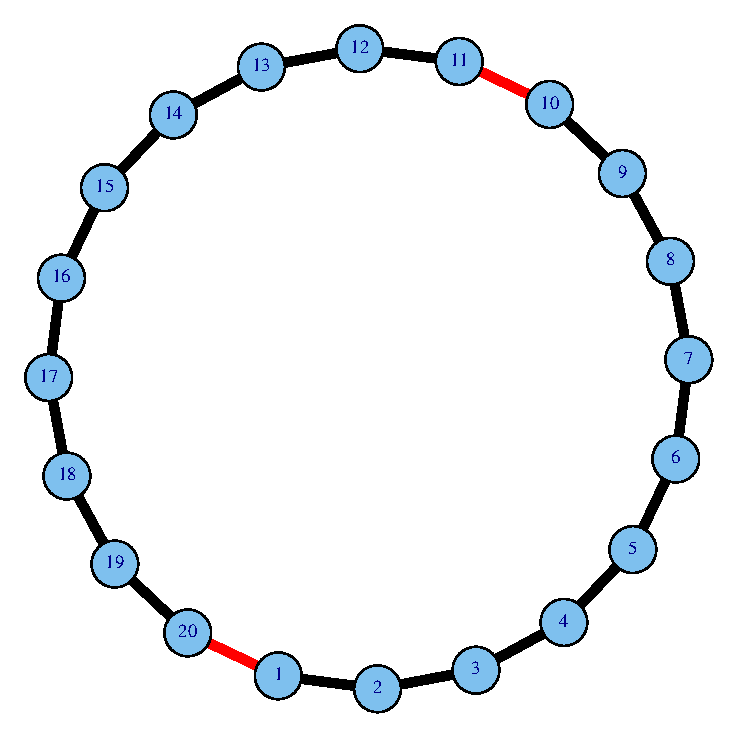
\includegraphics[scale=0.35]{ringGraph.eps}
%     \caption{A ring graph with $n=20$. If this graph is cut at the edges that are colored red, then $n/2$ vertices of the graph will be disconnected. Since a large fraction of graph can be separated with only two cuts, we say that this graph does not have ``good expansion''.}
%     \label{fig:ringGraph}
% \end{figure}
The results in this section relate graph invariants to the spectrum of the corresponding Laplacian matrix. The graph \textit{conductance} and the \textit{spectral expansion} are invariants that measure how much worse an arbitrary graph is compared to a clique. The \textit{spectral expansion} of a graph is defined as the second smallest eigenvalue of $L$. For the \textit{conductance}, consider a finite, simple, $d$-regular graph $\GD$. Choose a subset of the vertices, $S \subset \cVGD$, and define the cut $\partial(S)=\{uv: u\in S, v \not\in S\}$ to be the set of edges that have one endpoint in $S$ and one endpoint not in $S$. Then the \textit{conductance} of the set $S$ can be defined as 
\begin{definition}[Conductance \cite{Spielman2010}]\label{def:edgeexp}
Let $\GD$ be a finite, simple, $d$-regular graph and let $S \subset \cVGD$ be a subset of the vertices in $G_d$. Then the \textit{conductance} of $S$ is defined as
\begin{align}\label{eq:expS} 
\phi(S) = \frac{\mid \partial(S)\mid}{d\cdot \min\{\mid S \mid,\mid S^C\mid\}},
\end{align}
\end{definition}
where $S^C = \cVGD - S$. This notion can be extended to any set in $G_d$, leading to the combinatorial expansion of $G_d$
\begin{definition}[Graph Conductance \cite{Spielman2010}] \label{def:combexp} Let $\GD$ be a finite, simple, $d$-regular graph and let $S \subset \cVGD$ be a subset of the vertices in $G_d$. Then the \textit{conductance} of $G_d$ is defined by: 
\begin{align} \label{eq:expG}
\phi(G_d) := \min_{\emptyset \subset \mid S \mid  \subseteq \frac{n}{2}} \frac{|\partial (S)|}{d |S|}.
\end{align}
\end{definition}
%Please see the following site for graph conductance definition above: http://courses.cms.caltech.edu/cs139/notes/lecture10.pdf
Computing the cut that minimizes $\phi(G_d)$, \ie the optimal cut, by combinatorial approaches is an NP-hard problem \cite{Garey1990}. Fortunately, it is possible to approximate the optimal cut through spectral graph theory instead. In order to do this, however, there must be a relation between the spectral characterization of a graph and its conductance. The celebrated Cheeger inequality, which we now state, precisely establishes this relation. 
% Intuitively, the concept of edge expansion can be thought of in the following way. Consider a ring graph shown in Figure \ref{fig:ringGraph}. Deleting just two edges from the edge set of a ring graph leads to a disconnected graph. In particular, if the graph is cut at the right edges, then it is possible to disconnect $n/2$ vertices from the graph. Since cutting a small number of edges leads to a large number of vertices being disconnected in the graph, we say that the ring graph does not have ``good edge expansion''. Edge expansion is a combinatorial property of graphs that has been used to gauge graph connectivity and diameter (speed). 
\begin{theorem}[Cheeger's inequality] \label{thrm:cheeger}
Let $\GD$ be a finite, simple, $d$-regular graph with the normalized Laplacian matrix $L$ given by \ref{eq:normalizedLaplacian} and let $\lambda_2$ be the second smallest eigenvalue of $L$. Then we have
\begin{align}\label{eq:cheeger} 
\frac{\lambda_2}{2} \leq \phi(G_d) \leq \sqrt{2 \lambda_2}.	
\end{align}
\end{theorem}
\begin{proof}
The proof can be found in \cite{Chung97}
\end{proof}
% The Cheeger inequality establishes a relationship between the spectral expansion of any graph, $\lambda_2$, and its conductance, $\phi(G_d)$. If the graph spectrum is known, then it is easy to check whether or not the graph admits a sparse cut. Recall that Lemma \ref{lem:eigL} states that the number of times that zero appears in the spectrum of $L$ is precisely the number of connected components of $G_d$. It can be shown that when $\lambda_2 \approx 0$, then $\phi(G_d) \approx 0$ and that the second smallest eigenvalue $\lambda_2$ and the conductance of a graph are continuous approximations of one another \cite{Chung97}. We define the notion of an expander graph next
% In order to prove that a graph possess desirable expansion properties, one must show that the conductance of the graph is bounded below by a constant. By the Cheeger inequality, then, it is enough to prove that the second smallest eigenvalue $\lambda_2$ for the family of graphs is bounded from below instead. Usually it is easier to reason about the eigenvalues of a graph than about its conductance. 
% \begin{definition}[$\gamma$-expander Graph]\label{def:expander}
% Let $\GD$ be a finite, simple, $d$-regular graph and let $d, \delta \in \mathbb{N}$ and $\gamma \in \R$. Then we say $G_d$ is a $\gamma$-\emph{expander} if $\lambda_2(\delta)\geq \gamma, \quad \forall d\leq \delta$. 
% \end{definition}
%By analyzing the spectral properties of expander graphs it can be shown that they are essentially sparse graphs with the connectivity properties of complete graphs. \textcolor{red}{Can more be said here?} 
Given a cut, $\partial (S)$, we may define another quantity that represents the density of edges between the set $S$ and its complement, $S^c = \cVGD-S$. 
\begin{definition}[Edge Density of a cut \cite{Fallat2003}]\label{def:edgedensity} Let $\GD$ be a finite, simple, $d$-regular graph and let $S \subset \cVGD$ be a subset of the vertices of $G_d$ with cut $\partial(S)=\{uv: u\in S, v \not\in S\}$. Then the \textit{edge density} of a cut $\partial (S)$ is defined to be
\begin{align}\label{eq:edgedensity}
\rho (S) = \frac{\mid \partial(S) \mid}{\mid S \mid \mid S^c \mid}n.
\end{align}
\end{definition}
Furthermore, we have the following lemma that will be used subsequently.
\begin{lemma}[Fallat Inequality \cite{Fallat2003}]\label{lem:minedgedenalgconnect}
Let $\GD$ be a finite, simple, $d$-regular graph and let $S \subset \cVGD$ be a subset of the vertices of $G_d$ with cut $\partial(S)=\{uv: u\in S, v \not\in S\}$. The edge density (\ref{eq:edgedensity})
% \begin{align*}
% \rho (S) = \frac{\mid \partial(S) \mid}{\mid S \mid \mid S^c \mid}n
% \end{align*}
of any subset of the vertex set, $S \subset \cVGD$, satisfies $\lambda_2 \leq \rho(S)$;
which holds with equality for some cut $\partial (S)$ if the following conditions are satisfied: i) Each vertex $s \in S$ is adjacent to $d_1$ vertices in $S^c$ and each vertex $t \notin S$ is adjacent to $d_2$ vertices in $S$, and ii) $\frac{d_1}{d_2} = \frac{\mid S^c \mid}{\mid S \mid}$. The spectral expansion is then $\lambda_2 = \rho(S) = d_1+d_2$.
\end{lemma}
\begin{proof}
The reader is encouraged to consult \cite{Fallat2003} for the proof.
\end{proof}
\begin{figure}
    \centering
    \includegraphics[scale=0.2]{CoSpectralGraphs.pdf}
    \caption{Two regular graphs with the same Laplacian matrix spectrum \cite{Brouwer2011}.}
    \label{fig:cospectral}
\end{figure}
% It has been shown that matrix spectra do not uniquely determine graphs. For example, the two graphs in Figure \ref{fig:cospectral} are both 4-regular and share the same Laplacian and adjacency spectrum. However, they are not isomorphic graphs since the one on the right has more triangles than the one on the left. This line of reasoning leads us to establish results to relate graph invariants such as the number of triangles to the graph spectrum. 
% \begin{theorem}[Spectral Expansion \& the third moment of $G$]\label{thrm:algTriangle}
% Let $G = (\cV, \cE)$ be a simple undirected connected graph with $n$ vertices and $m$ edges. Then, 
% \begin{align} \label{eq:nazInequality}
% \frac{2m - R}{n-1} \leq \lambda_2 \leq \frac{n \displaystyle\sum_{i \in \cV}d_i^2 - 6n\triangle(G)}{2mn - \displaystyle\sum_{i \in \cV} d_i^2}.
% \end{align}
% where $\triangle(G)$ is the number of triangles in $G$ and
% \begin{align*}
% R = \sqrt[]{(n-2)\left ((n-1)\displaystyle\sum_{i \in \cV}d_i^2 + 2m(n-2m-1)\right)}.
% \end{align*}
% \end{theorem}
Using Lemma \ref{lem:minedgedenalgconnect} we prove a new result relating the spectrum of the adjacency matrix to the third moment of a graph. In order to motivate the result, recall that it has been shown that matrix spectra do not uniquely determine graphs \cite{God2001}. For example, the two graphs in Figure \ref{fig:cospectral} are both 4-regular and share the same Laplacian spectrum. However, they are not isomorphic graphs since the graph on the right contains more triangles than the one on the left. To our knowledge this result has not been reported in the intrusion detection literature. 
\begin{theorem}[Spectral Expansion \& The Moments of $M$]\label{thrm:algTriangle}
Let $G = (\cV, \cE)$ be a finite, simple, connected graph with $n$ vertices and $m$ edges. Then, 
\begin{align} \label{eq:nazInequality}
\frac{2m - R}{n-1} \leq \lambda_2 \leq \frac{n \displaystyle\sum_{i \in \cV}d_i^2 - 6n\triangle(G)}{2mn - \displaystyle\sum_{i \in \cV} d_i^2}.
\end{align}
where $\triangle(G)$ is the number of triangles in $G$ and $R = \sqrt[]{(n-2)\left ((n-1)\sum_{i \in \cV}d_i^2 + 2m(n-2m-1)\right)}$.
\end{theorem}
\begin{proof}
First we show $\frac{2m - R}{n-1} \leq \lambda_2$. The diagonal elements of $L$ and $L^2$ are $d_i$ and $d_i^2+d_i$ respectively. Now, $\sum_{i \in \cV} d_i = 2m$ and $\sum_{i \in \cV}(d_i^2 + d_i) = \sum_{i \in \cV} d_i^2 + 2m$. Using the Cauchy-Schwarz inequality, one can show that $\sum_{i \in \cV} (d_i^2 + 2m) - \lambda_2^2 \geq \frac{(2m-\lambda_2)^2}{n-2}$. Rearranging the terms will produce $\frac{2m - R}{n-1} \leq \lambda_2$ as desired. Next we show that $\lambda_2 \leq \frac{n \sum_{i \in \cV}d_i^2 - 6n\triangle(G)}{2mn - \sum_{i \in \cV} d_i^2}$. Note that, by Lemma \ref{lem:minedgedenalgconnect}, $\lambda_2 \leq \rho(S)$. Let $S = \cN_i$. Observe that $\mid \partial (\cN_i) \mid = \sum_{j \in \cN_i} d_j - 2\triangle(i)$, where $\triangle(i)$ denotes the number of triangles that vertex $i$ participates in. Now, Lemma \ref{lem:minedgedenalgconnect} can be stated as $\lambda_2 \mid \cN_i \mid \mid V - \cN_i \mid \leq n \mid \partial(\cN_i) \mid$.
But the quantity $\mid \cN_i \mid \mid V - \cN_i \mid$ can be written as $d_i (n-d_i)$. Therefore, we have $\lambda_2 d_i (n-d_i) \leq n\sum_{j \in \cN_i} d_j - 2\triangle(i)$.
Hence, by summing over all the vertices in the graph, one obtains the desired result.
% \begin{align*}
% \lambda_2 \leq \frac{n \sum_{i \in \cV}d_i^2 - 6n\triangle(G)}{2mn - \sum_{i \in \cV} d_i^2}
% \end{align*} 
% Then $\displaystyle \lambda_2 \leq \displaystyle\frac{\mid \partial (\cN_i)\mid }{\mid \cN_i \mid \mid V - \cN_i \mid}n = \displaystyle\frac{\mid \partial (\cN_i)\mid }{d_i (n-d_i)}n$.
\end{proof}
%\subsection{Distributed System Model} There are many ways to model the dynamics of a distributed system. Our formulation does not assume any particular modeling approach. One exemplary approach is provided below.  
% \subsubsection{Nominal System Behavior} Consider a group of $n$ agents with single integrator dynamics 
% \begin{align*}
% \dot{x}_i &= u_i, \\
% y_i &= x_i 
% \end{align*}
% that have an initial condition $x_i (0) = x_{i0} \in \mathbb{R}$ and that are connected through a communications network which can be modeled by an undirected graph, $G$. Let the distributed control law
% \begin{align*} 
% \displaystyle u_i = \sum_{j \in \mathcal{N}_i} (x_j - x_i)
% \end{align*}
% be assumed; where $u_i$ is the control input to agent $i \in \mathcal{V}$, $x_i \in \mathbb{R}$ is the state of agent $i$ and $x_j \in \mathbb{R}$ is the state of one of agent $i$'s neighbors. In the nominal case (there are no intruders), the model 
% \begin{gather} 
% \begin{aligned} \label{eq:agentCons}
% \dot{x}_i &= \sum_{j \in \mathcal{N}_i} (x_j - x_i) \\
% y_i &= x_i
% \end{aligned}
% \end{gather}
% is in effect for each agent $i \in \mathcal{V}$. Under these assumptions, the collective dynamics of the entire network are given by:
% \begin{align} \label{eq:consensysDyn}
% \dot{\mathbf{x}} = -L\mathbf{x}
% \end{align}
% where $L \in \mathbb{R}^{n \times n}$ is the graph Laplacian of $G$ and $\mathbf{x} \in \mathbb{R}^n$ is the state vector. 

% In a distributed system, each agent $i \in \mathcal{V}$ only has access to the states of the $m$ agents in its local neighborhood, $\mathcal{N}_i$. Let, the set of states available to agent $i \in \mathcal{V}$ be defined by:
% \begin{align} \label{eq:Ci}
% w_i = \left [ \begin{array}{ccc} x_{i_1},&\ldots,&x_{i_{|\mathcal{N}_i}|} \end{array}\right ]^T = C_i \mathbf{x}
% \end{align}
% where $C_i \in \mathbb{R}^{m \times n}$ encodes the interconnection topology of agent $i \in \mathcal{V}$. 
% \subsubsection{Modeling Malicious Agents} In the presence of intruders, the system model for the agent that is the target of an intruder must be modified since it no longer updates its state correctly. Instead, if agent $j \in \mathcal{N}_i$ is the target of an intruder, then it may update its state according to:
% \begin{gather} 
% \begin{aligned} \label{eq:agentConsFaultAct}
% \dot{x}_j &= \sum_{i \in \mathcal{N}_j} (x_i - x_j)+f_j \\
% y_j &= x_j
% \end{aligned}
% \end{gather}
% where $f_j$ is a function of time that is introduced by an intruder. The network dynamics become:
% \begin{gather} \label{eq:globalDynActFault}
% \begin{aligned} 
% \dot{\mathbf{x}} &= -L\mathbf{x}+b_j f_j \\
% \mathbf{y} &= \mathbf{x} 
% \end{aligned}
% \end{gather}
% where $b_j \in \mathbb{R}^n$ is a vector with the $j$th component(s) set to 1 and all others zero. If, instead, the communications channels of agent $j$ are targeted, the model becomes:
% \begin{gather} 
% \begin{aligned} \label{eq:agentConsFaultSen}
% \dot{x}_j &= \sum_{i \in \mathcal{N}_j} (x_i-x_j) \\
% y_j &= x_j + f_{j}
% \end{aligned}
% \end{gather}
% and the network dynamics become
% \begin{gather} 
% \begin{aligned} 
% \dot{\mathbf{x}} &= -L\mathbf{x}+I_{\bar{j}}l^j f_j \\
% \mathbf{y} &= \mathbf{x}+b_j f_j
% \end{aligned}
% \end{gather}
% where $I_{\bar{j}} \in \mathbb{R}^{n \times n}$ is the identity matrix with the $j^{th}$ diagonal entry set to zero, $l^j \in \mathbb{R}^n$ is the $j^{th}$ column of the Laplacian matrix. Now we precisely define a malicious agent:
% \begin{definition}
% (Malicious or Faulty Agent): Agent $j \in \mathcal{N}_i$ is said to be a \textit{malicious} or \textit{faulty} agent if $f_j \neq 0$ in (\ref{eq:agentConsFaultAct}) or (\ref{eq:agentConsFaultSen}) for any time. 
% \end{definition}
% %\begin{remark}
% %We do not assume any form for the function $f_j$. 
% %\end{remark}
% \begin{remark} \label{rem:rem1}
% Based on the definition of a malicious agent one may observe that from the perspective of agent $i \in \mathcal{V}$, a communications attack on agent $j \in \mathcal{N}_i$ and a direct attack on agent $j\in \mathcal{N}_i$ are indistinguishable. This observation was also reported in \cite{Teix2010} and we will continue to adopt it in this paper. 
% \end{remark}
% \subsubsection{Modeling the Monitoring Agents}
% In our model, the network is equipped with a set of agents that monitor their neighbors for intrusions. Since every agent in the network has access to the information flow from its neighbors, any agent may be assigned the task of sensing for malicious intrusions in the network. Our distributed model consists of endowing each of these agents with a carefully designed filter so that intruders in their neighborhood can be distinctly identified. We give the following definition for such agents:
% \begin{definition}
% (Monitoring Agent): Let $G_i \triangleq (-L-D_i C_i)$. Then, agent $i \in \mathcal{V}$ is said to be a \textit{monitoring agent} if it is endowed with a detection filter of the form:
% \begin{gather}\label{eq:luenObsAgent}
% \begin{aligned} 
% \dot{\hat{x}}_i &= G_i\hat{x}_i +D_i y_i \\
% \hat{y}_i &= C_i\hat{x}_i.
% \end{aligned}
% \end{gather}
% and a detection gain, $D_i$, such that the residual
% \begin{align} \label{eq:residual}
% r_i = y_i-\hat{y}_i
% \end{align}
% has a fixed direction associated with each of the $j \in \mathcal{N}_i$ neighbors of $i \in \mathcal{V}$ when they are under attack.  
% \end{definition}
% \subsection{Distributed Detection Filter Design} \label{sec:sec3} The monitoring agents in the distributed system that form $H$ are endowed with detection filters. Our approach does not require a particular detection filter structure, however we provide an exemplary detection filter below for convenience. 
% The conditions under which a solution exists for the detection gain $D_i$ are given in Theorems \ref{thrm:distributedDetection} and \ref{thrm:distributedDetectionNonDistinct}. These conditions are formulated in terms of local agent interactions and the desired spectral characteristics of the detection filter. The proofs of the main results provide insight into a procedure that can be used to obtain the detection filter gains. Briefly, this consists of constructing a linear system of equations whose solution gives the desired filter gains for an interaction topology and a specified eigenstructure. 

% Let agents $i$ and $j$ be the monitoring and malicious agents, respectively. The main result of this section addresses the problem of identifying which of the $k$ agent(s) in the set $\mathcal{N}_i$ are malicious agents.   

% \begin{definition} (Intruder Detectability)
% Let $\epsilon_i = x_i-\hat{x}_i$ be the state estimation error of monitoring agent $i \in \mathcal{V}$. A malicious agent $j \in \mathcal{N}_i$ is \textit{detectable} by a monitoring agent $i \in \mathcal{V}$ if there exists a filter gain $D_i$ such that $r_i = C_i \epsilon_i$ maintains a fixed direction in the output space and all eigenvalues of $G_i$ can be almost arbitrarily placed. 
% \end{definition}

% \begin{remark}
% In this paper we do not consider the class of signals for which $r_i$ does not posses directional properties. 
% \end{remark}

% The assumptions under which detection filter theory is valid must be extended to the distributed case. Here, they are captured in terms of the interconnection topology of the graph that models the distributed system:
% \begin{ass} \label{ass:distEigen} Let agent $i \in \mathcal{V}$ be a monitoring agent and let agent $j \in \mathcal{N}_i$ be a malicious agent. Then we assume that 
% \begin{itemize}
% 	\item the pair $(-L,C_i)$ is observable.
%     \item the vector $C_i b_j \neq \underline{0} \quad \forall j = 1,2,\ldots, m$.
%     \item the $rank(C_i F) = m$, where $C_i F = \left [C_i b_1, \ldots, C_i b_m \right ]$ and $m=|\mathcal{N}_i|$.
%  \end{itemize}
%  \end{ass}
 
%  \begin{remark} The condition $rank(C_i F)=m$ in assumption \ref{ass:distEigen} is known as \textit{output separability}.  When $m=|\mathcal{N}_i|$, then the maximum number of malicious agents are detectable. Note that this assumption can be relaxed and the theory is still valid \cite{White1987}. 
%  \end{remark}
 
% Throughout this paper, we assume that the monitoring agent $i \in \mathcal{V}$ has access to the fixed network topology through the graph Laplacian matrix $L$ and that there is no uncertainty in the monitoring agent and malicious agent models (as given in section (\ref{sec:sec2})). The following lemma is needed to prove the main results. 

% Let $\left \{\lambda_l^i \right\}_{l=1}^n$ be the distinct eigenvalues of $G_i$ and let $\{V_l^i\}_{l=1}^n$ be an associated set of eigenvectors. Then we have the eigenvalue-eigenvector equation:
%  \begin{align} \label{eq:eq0}
%  \left (\lambda_l^i I - G_i \right ) V_l^i = 0 \quad \forall l = 1, \ldots, n.
%  \end{align}
% Next, let us write the vector $b_j$ as a linear combination of the eigenvectors of $G_i$:
%  \begin{align} \label{eq:fjLinComb}
%  b_j = \sum_{l=1}^{n_j} \alpha_l^j V_l^i, \quad n_j \leq n.
%  \end{align}
%  and define the controllability matrix of $b_j$ to be: 
%  \begin{align} \label{eq:wj}
%  W_j = \left [b_j, G_i b_j, \ldots, G_i^{n-1}b_j \right],
%  \end{align}
% whose columns define the controllable space of the attack direction $b_j$ with respect to the matrix $G_i$. 

%Now we are ready to state the main result of the memo. The following result can be used to choose the detection gain, $D_i$, so that agent $i$ is able to simultaneously detect multiple intruders within its $|\mathcal{N}_i|$ neighborhood.

% \begin{lemma} \label{lem:distributedDetection}
% Given a distributed system having the undirected graph $G(\mathcal{V},\mathcal{E})$, with consensus dynamics given by

% \begin{align} \label{eq:conDyn}
% \dot{x} = -Lx,
% \end{align}
% a monitoring agent $i \in \mathcal{V}$ with detection filter
% \begin{gather}\label{eq:detFilter}
% \begin{aligned} 
% \dot{\hat{x}}_i&=G_i\hat{x}_i + D_i y_i \\
% \hat{y}_i &= C\hat{x}_i
% \end{aligned}
% \end{gather}
% will detect and identify any intruder agent(s) $j \in \mathcal{N}_i$ if and only if
% \begin{cond} \label{num:cond1}
% $C_i b_j = C_i V_l^i \quad \forall j,l = 1,\ldots,k \quad$  
% \end{cond}
% \begin{cond} \label{num:cond2}
% $\sum_{j=1}^m null(M_j) = k$.
% \end{cond}
% \noindent where $null(M_j)$ denotes the nullity of $M_j$, $k \leq m$, and 
% \begin{align}
% M_j &= \left [ \begin{array}{c} \gamma_j \\ \gamma_j A_j \\ \vdots \\ \gamma_j A_{j}^{n-1} \end{array} \right ] \label{eq:eq3}\\
% \gamma_j &= \left [ I - C_i b_j (C_i b_j)^{\dagger}\right]C_i \label{eq:eq4}\\
% A_j &= -L\left [I - b_j(C_ib_j)^{\dagger}C_i\right ] \label{eq:eq5}\\ 
% G_i &= (-L-D_iC_i). \nonumber
% \end{align}

% \noindent Furthermore, for a given set of distinct eigenvalues, $\{ \lambda_l^i \}$, the detection gain, $D_i$, and the desired eigenvectors, $V_l^i$, are given by the following linear system of equations:
% \begin{align} \label{eq:linSystem}
% \left [ \begin{array}{cc} \lambda_l^i I + L & D_i \\ C_i & 0 \end{array} \right ]\left [ \begin{array}{c} V_l^i \\ C_i V_l^i \end{array}\right] = \left [ \begin{array}{c} 0 \\ C_i b_j \end{array} \right ].
% \end{align}
% \end{lemma}
% The linear system in Lemma \ref{lem:distributedDetection} provides a way to design the detection filters so that every intruder in the neighborhood can be isolated. However, the result does not give insight into the strategy for choosing the monitoring agents from among the $n$ agents in $G$. In the next section, we argue that one approach is to choose a subset of the vertices $S \subset V$ such that the induced graph on $S$ forms an expander graph. In other words, we argue that the subgraph $H$ induced by the monitoring agents that is maximally robust to adversarial attacks possesses the largest spectral expansion of any subgraph in $G$. The subgraph $H$, chosen such that it has the largest spectral expansion, gives the overall detection scheme the best expansion properties. This makes the network of monitoring agents maximally robust to intruder attacks. This is a well known result in graph theory \cite{Wig2006,Lub2012,Lub1988}. Furthermore, the robustness of the graph to attacks can be quantified by $\lambda_2 (L)$ or $\lambda_2 (H)$. Additionally, Teixeiras results for reducing the computational complexity of the monitoring agents is 1) not robust, i.e. any minimization over the vertex set recovery problem may not have good expansion properties and 2) is plagued by time complexity...it is NP-hard. Our approach is 1) maximally robust to attacks and 2) can be computed in polynomial time.  
% %-----------Problem Formulation-----
\section{Problem Formulation \& Spectral Recovery} \label{sec:problemFormulationSpecRecovery}
Recall that in section \ref{sec:Prelim} a relationship between a graph invariant known as the graph conductance and a graph cut was defined. As noted \textit{supra}, the graph conductance is a quantity that relates its reliability and diameter in a useful way. In intrusion detection applications, we exploit this result to quantify the resiliencey of a network of monitoring agents in the presence of adversarial attacks. The next result establishes a connection between the graph conductance and an attack on the edge set of a graph by an adversary.
\begin{lemma} \label{lem:adversaryConComp}
Let $\GD$ be a finite, simple, $d$-regular graph of conductance $\phi$. Then after an attack by an external adversary on $\epsilon < \phi$ fraction of its edge set, the graph $G_d$ will still have a connected component of at least $(1-\epsilon/2\phi)$ fraction of the vertices. 
\end{lemma}
\begin{proof}
Choose an arbitrary subset of the edges $\cEGD' \subseteq \cEGD$ such that $\cEGD' \leq \epsilon \cEGD$. Recall that $G_d$ is $d$-regular, therefore we can write $\cEGD' \leq \epsilon\frac{dn}{2}$. Define the following ordered partition on $G_d$: $|\cC_1| \geq |\cC_2| \geq \ldots \geq |\cC_m|$. We seek to show that the largest partition, $|\cC_1|$ satisfies $|\cC_1| \geq (1-\frac{\epsilon}{2\phi})n$. Note that $\cEGD'$ is at least half the edge boundaries. To see this, consider $\frac{1}{2} \sum_i |\partial(\cC_i)| \leq |\cEGD'| \leq \epsilon\frac{dn}{2}$. If $|\cC_1| \leq \frac{n}{2}$, then it is easy to see that $\epsilon \leq \phi$, a contradiction. Therefore, $|\cC_1| \geq \frac{n}{2}$. Define $\cS := \cC_2 \cup \ldots \cup \cC_m$. We have $d\phi |\cS| \leq |\partial(\cC_1)| \leq \epsilon\frac{dn}{2}$.Therefore, $|\cS| \leq \frac{\epsilon}{2\phi}n$. But we have already shown that $|\cC_1| > |\cS|$.  Therefore, we must have $|\cC_1| >\left(1- \frac{\epsilon}{2\phi} \right)n$.
\end{proof}
As previously discussed, computing the graph conductance is an NP hard problem, scoping the utility of lemma \ref{lem:adversaryConComp}. Instead, we can address the problem of ascertaining the maximally resilient monitoring network through spectral means. 
% Expander graphs are simultaneously sparse and highly connected making them a class of graphs for which it is difficult to disconnect a large part of the graph without severing a large fraction of the edge set. The graph isoperimetric number captures the notion that every set of vertices in a expander graph has a large neighborhood, a property that is naturally related to connectivity. Given these connectivity properties, it is surprising that expanders are `sparse', i.e. they have a low average vertex degree. Furthermore, these combinatorial properties are related to the graph Laplacian spectrum by the Cheeger Inequalities. Generally speaking, the spectral expansion (also known as the algebraic connectivity) of $G$ determines its connectivity properties, including whether or not $G$ contains sparse cuts. 
Let $\GD$ be a finite, simple, $d$-regular graph that models an underlying distributed system. Denote a subgraph of $G_d$ over the vertex subset $\cV \subseteq \cVGD$ by $G[\cV]$. Denote the Laplacian matrix of $G[\cV]$ by $L_{\cV}$. Let $\lambda_2(\cV)$ denote the second largest eigenvalue of $L_{\cV}$. We seek the largest subgraph of $G_d$ with maximum spectral expansion. More formally, we have the following optimization problem over the vertices of $G_d$
% \begin{align}
% |\cV |\geq \delta n \label{eq:specSize}
% \end{align} 
% and spectral expansion
\begin{align}
% \displaystyle \lambda(\delta) = \max_{\cV:|\cV| \geq \delta n} \quad \lambda_2(\cV).
% \end{align} \label{eq:specExp}
\displaystyle \lambda = \max_{\cV:|\cV| \geq \delta n} \quad \lambda_2(\cV). \label{eq:specExpansion}
\end{align} 

% \textcolor{red}{Equation \ref{eq:specExpansion} can be interpreted in the following way: choose any subset of the vertices that satisfies the condition in $\ref{eq:specSize}$. Then, construct the Laplacian matrix associated with the induced graph given by $\cV$ and its corresponding edge set, $\cE$. Next, compute the second eigenvalue of the Laplacian matrix associated with this subgraph. Then, the set of vertices with the largest spectral expansion are the maximizers of \ref{eq:specExpansion}.}  
% Relatedly, it can be shown that the most vulnerable agents in the network belong to the set $\cV_T \subset \cV_G$, with edge expansion: 
% \begin{align}
% %h(\delta) =
% \displaystyle \min_{\cV_T:|\cV_T| \leq \delta n} \quad h(\cV_T).
% \end{align}
% %-----------Main results------------
%\section{Spectral Recovery} \label{sec:spectralRecovery}
% First we show that the upper bound of the algebraic connectivity of a graph is a function of the number of triangles $t(G)$ and then we prove a result that gives the conditions to recover the largest hidden expander $H$ in $G$. A spectral recovery algorithm is provided as well. In the next section, we give two design procedures for $H$. The design procedures can be used if explicit constructions of $H$ are required, i.e. Algorithm \ref{alg:alg1} does not produce a feasible solution.
 We address the problem in \ref{eq:specExpansion} under the constraint that the edge set of $G$ cannot be altered to accommodate the monitoring agents. 
\begin{theorem} \label{thrm:existenceOfH}
Let $G_d=(\cV_{G_d}, \cE_{G_d})$ be a $d$-regular network of $n$ agents under consensus and let $0<\delta <1$ be a parameter representing the fraction of agents in $G_d$ that will be chosen as monitoring agents. Then there exists a monitoring graph $H_d$ with at least $|\cV_{H_d}| > \frac{3}{8} \delta n$ agents forming a topology with spectral expansion $\lambda_2 (\cV_{H_d}) > \frac{\lambda^2 \delta^2}{32d(log^2 \delta)}$.

\end{theorem}
\begin{proof}
First we show that for a finite, simple, $d$-regular graph $G_d$ with parameters $0<\gamma, \delta < 1$ there exists a set $\cV_{H_d} \subseteq \cV_{G_d}$ of size $\frac{3}{8}\gamma n$ and spectral expansion $\lambda_2 (\cV_{H_d}) \geq \gamma d$, or a partition of $\cV_{G_d}$, denoted by $\cP$ into sets of size at most $\frac{\delta n}{2}$ such that
\begin{align}
\sum_{\cT \in \cP} |\partial (\cT)| \leq 2dn\left(log\frac{1}{\delta}\right)\sqrt[]{2\gamma} \label{eq:property}
\end{align}
To see this, we refer to algorithm \ref{alg:alg1} and note that when $\lambda_s(\cVGD) \geq \gamma d$, then the proof is complete. When $\lambda_s (\cVGD) < \gamma d$, then it is possible to partition $\cVGD$ into two pieces using algorithm \ref{alg:alg1} for a given $\gamma$. If algorithm \ref{alg:alg1} is applied to each partition recursively, then eventually either $\lambda_2(\cVGD) \geq \gamma d$ or all partitions within $G_d$ will have size at most $\frac{\gamma n}{2}$. If an expander is found, its size is at least $\frac{3 \gamma n}{8}$. If an expander is not found, then there exists $\cP$ partitions of $\cVGD$ with the property \ref{eq:property}. To see this, let $l_i = \sum_{\cT \in \cP_i} |\partial (\cT)|$ where the index $i$ denotes the index of the set at the end of the iteration $i$. Note that $l_i \leq l_{i-1} + dn\sqrt[]{2\gamma},\forall i>1$. The justification for this being that each $\cP_i$ is obtained by splitting all sets in $\cP_{i-1}$ into two new sets by a cut of expansion at most $d\sqrt[]{2\gamma}$. Also, it can be shown that algorithm \ref{alg:alg2} converges in at most $2log\left(\frac{1}{\delta}\right)$ iterations (since $1/2^{n/2}=\gamma$) \cite{Algs2001}. Therefore, we have $\sum_{\cT \in \cP} |\partial(\cT)| \leq 2dn\left(log\frac{1}{\delta}\right)\sqrt[]{2\gamma}$ which is the property \ref{eq:property}. Now suppose that for some $\gamma$ algorithm \ref{alg:alg2} produces a partition $\cP$ of $\cVGD$ into sets of size at most $\frac{\delta n}{2}$ with $\sum_{\cT \in \cP} |\partial(\cT)| \leq 2dn\left(log\frac{1}{\delta}\right)\sqrt[]{2\gamma}$.  It is easy to see that $\sum_{\cT \in \cP} |\partial(\cT)| \geq \sum_{\cT \in \cP} |\partial(\cT \cap \cVHD)| \geq \sum_{\cT \in \cP} \frac{\lambda}{2} |\cVHD \cap \cT| \geq \lambda_2 \delta n$. Therefore, $\frac{\lambda}{2} \delta n \leq 2dn\left(log\frac{1}{\delta}\right)\sqrt[]{2\gamma}$. With some algebra, we can now show that 
\begin{align}
\gamma d \geq \frac{\lambda^2 \delta^2}{32dlog^2(\delta)}. \label{eq:gammad}
\end{align}
Finally, using \ref{eq:gammad} it is easy to see that $\lambda_2 (\cVHD) \geq \gamma d \geq \frac{\lambda^2 \delta^2}{32dlog^2(\delta)}$ which completes the proof. 
\end{proof}
Furthermore, to extract the hidden subgraph of monitoring agents from within $G$, one can  recursively apply the spectral bisection algorithm listed in Algorithm \ref{alg:alg1}. As shown in Algorithm \ref{alg:alg2}, repeated spectral bisections of $G$ will lead to the  induced expander $H$.
\begin{algorithm} 
    \SetKwInOut{Input}{Input}
    \SetKwInOut{Output}{Output}

    %\underline{function Euclid} $(a,b)$\;
    \Input{A graph $G=(V,E)$, with any vector $l \in \R^{\cV}$}
    \Output{A cut $\partial (S)$ in $G$ and $k \in \N$}
    Sort the vertices of $G$ according to the values of $l$. \\ 
    Find a $k \in \N$ that minimizes $h(\{v_1,\ldots,v_k\},\{v_{k+1},\dots,v_n\})$ and output the index $k$ of $v_k$. 
    \caption{Spectral Partitioning Algorithm}\label{alg:alg0}
\end{algorithm}
\begin{algorithm} 
    \SetKwInOut{Input}{Input}
    \SetKwInOut{Output}{Output}

    %\underline{function Euclid} $(a,b)$\;
    \Input{A graph $G[\cV]$ with maximum degree $d$ and $0 < \gamma < 1$.}
    \Output{A set $\cV_H$ such that, either $|\cV_H| \geq \frac{3}{4}n$ and $\lambda_2 (\cV_H) \geq \gamma d$, or $\frac{n}{4} \leq |\cV_H| \leq \frac{3}{4}n$ and $h(\cV_H) \leq \sqrt{2\gamma}d$ }
    Let $\cV_H=\cV_G$. \\ %\eIf{$b=0$}
    \While{$|\cV_H| \geq \frac{3}{4}n$}
    	{If $\lambda_2 (\cV_H) \geq \gamma d$ then \Return{$\cV_H$}.\\ Otherwise, run the spectral partitioning on $H$ and let $(T,\cV_H \setminus T)$ be the output. \\ Say $|T| < |\cV_H \setminus T|$. Let $\cV_H = \cV_H \setminus T$.}
 	\Return{$\cV_G \setminus \cV_H$}
    \caption{Spectral Bisection Algorithm}\label{alg:alg1}
\end{algorithm}
\begin{algorithm} 
    \SetKwInOut{Input}{Input}
    \SetKwInOut{Output}{Output}
    \Input{A graph $G$ with maximum degree $d$ and parameters $0 < \delta,\gamma < 1$.}
    \Output{A subset of $\cV_H$ or a partitioning of it, $\mathcal{P}$.}
    Let $\mathcal{P}=\{\cV_G\}$. \\ %\eIf{$b=0$}
    \While{there is a set in $\mathcal{P}$ with more than  $\frac{\delta n}{2}$ vertices}{
    	\ForAll{$\cV \in \mathcal{P}$ with $|\cV|>\frac{\delta n}{2}$ vertices}{
        Run Algorithm \ref{alg:alg1} on input $\gamma$ and $G[\cV]$. Let $\cV_H \subseteq \cV$ be the output. \\
        If $\lambda_2(\cV_H) \geq \gamma d$, return $\cV_H$. Otherwise, add $\cV_H$ and $\cV\setminus{\cV_H}$ to $\mathcal{P}$ and remove $\cV$.\label{line:elseline}}
        }
    \Return $\mathcal{P}$.\label{line:nonexpanding}
    \caption{Resilient Monitoring Network}\label{alg:alg2}
\end{algorithm}
% %-----------Illustrative Example------------
\section{Illustrative Example} \label{sec:Example}
This example will consider the diameter, connectivity and spectral expansion for a network that was recently addressed by the authors of \cite{teixeira_distributed_2014}. This network is reproduced in Figure \ref{fig:TeixierasNetworkCut} for convenience. Table 1 lists the network diameter, connectivity and spectral expansion of $G_T$. Figure \ref{fig:TeixierasNetworkH} shows the network of monitoring agents $H_T$ formed by the proposed proximity method of \cite{teixeira_distributed_2014}. The graph diameter, connectivity and spectral expansion for $H_T$ have also been tabulated in Table 1. Notably, the spectral expansion has increased in $H_T$ (from $0.125$ to $0.184$), implying that the network of monitoring agents is more resilient to network attacks than the original graph $G_T$. However, $H_T$ is still a 'slower' network with a diameter of $4$ and half as reliable as $G_T$ with a connectivity of $1$. Next we use algorithm 3 to construct the network of monitoring agents, $H$. We specify $\delta = 1.6$ to obtain a network of monitoring agents with a minimum of $|\cV_H|=7$ agents and we specify $\gamma = 2\lambda_2 (G_T)$ $\ie$ we require that the network of monitoring agents have a spectral expansion of at least twice $G_T$. Algorithm 3 executes in under $500 \mu sec$ and returns the vertices $\cV_H = \{1,2,3,4,5,6,7\}$. This is the resilient network of monitoring agents as shown in Figure \ref{fig:OurProposal} with network diameter, connectivity and spectral expansion tabulated in Table 1. Notably, the spectral expansion of $H$ is $0.320$, a large improvement over $H_T$. The network diameter is better with a figure of $3$ and the network reliability is back up to $2$. Therefore, $H$, the network of monitoring agents recovered by algorithm \ref{alg:alg2} is more resilient than $H_T$. 
% Next, the network of monitoring agents $R_H$ is constructed according to Theorem \ref{thrm:ramanujanAgents}. In this case, the network of monitoring agents is not constrained by the edge set of the original graph. It is assumed that the design can be altered so that a subnetwork of monitoring agents can be constructed with the only constraint being that the monitoring agents are constrained to a neighborhood set with cardinality at most three. The network is shown in Figure \ref{fig:RamanujanAgents}. The network diameter, connectivity and spectral expansion are tabulated in Table 1. The spectral expansion in this case is $0.350$, which is larger than $H_T$ and $H$. Furthermore, the diameter and connectivity properties of $R_H$ are superior to $H_T$ and $H$ as well. 
\begin{figure}
\begin{subfigure}{.2\textwidth}
  \centering
  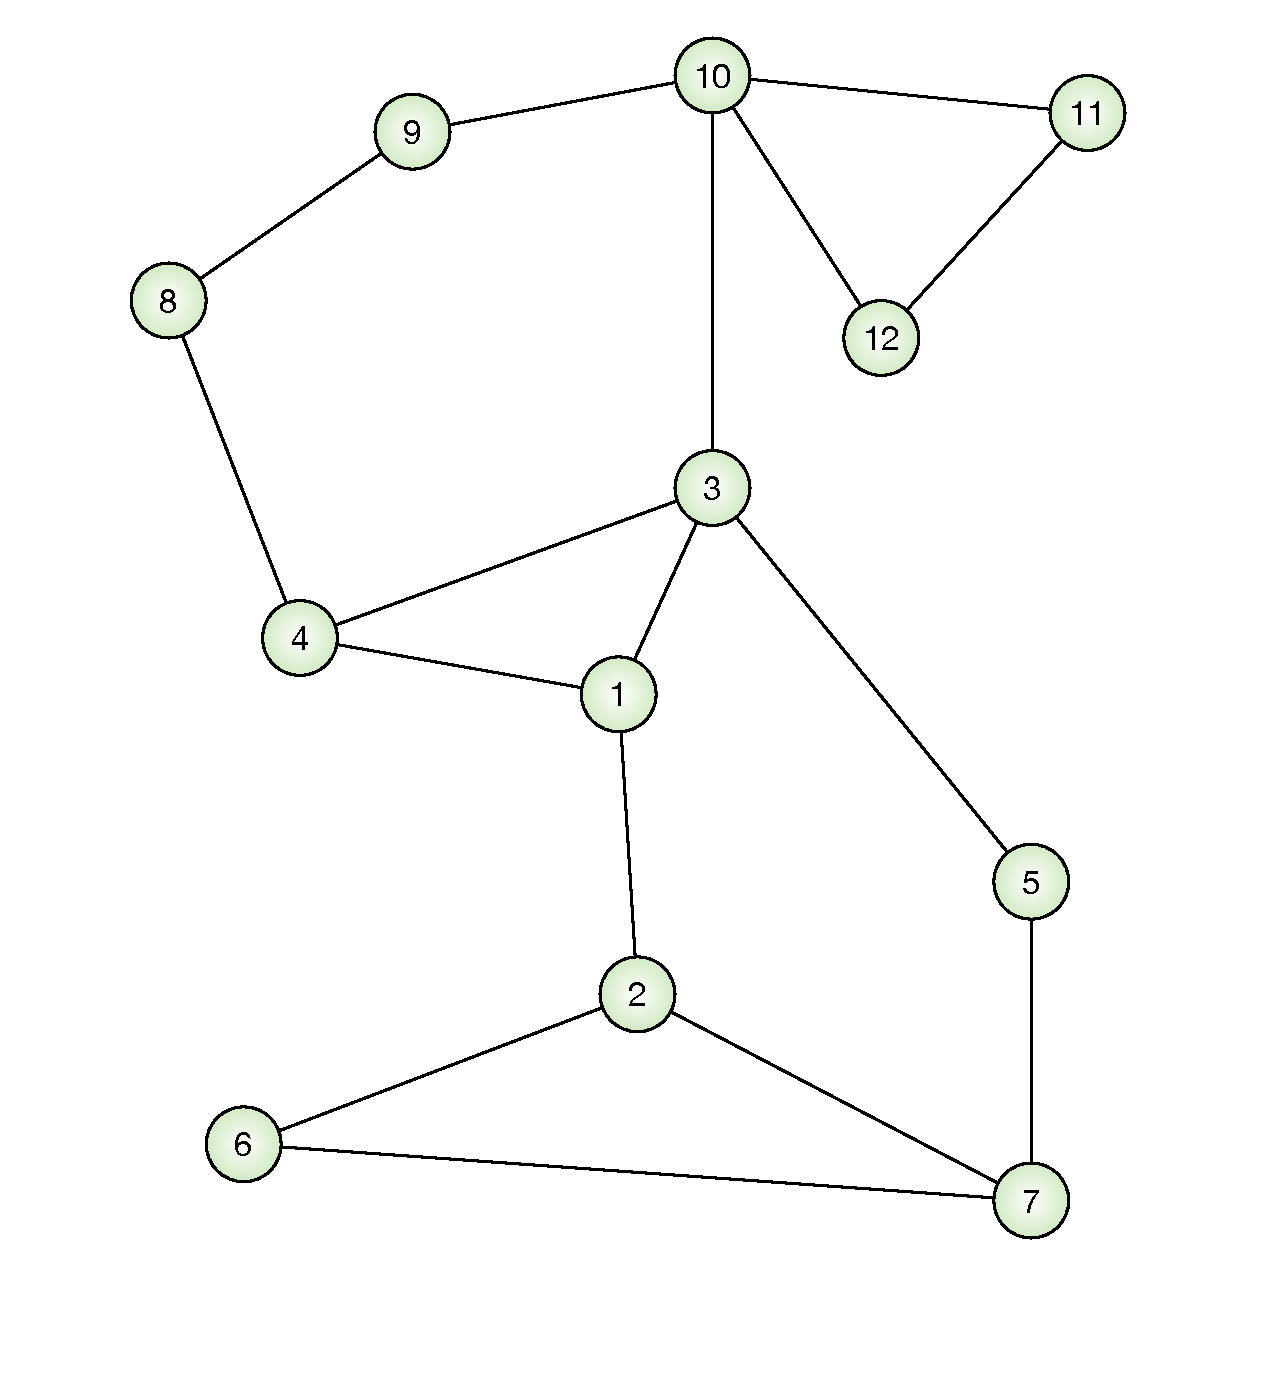
\includegraphics[width=.8\linewidth]{teixieraNetwork2014.pdf}
  \caption{$G_T$}
  \label{fig:TeixierasNetworkCut}
\end{subfigure}%
\begin{subfigure}{.2\textwidth}
  \centering
  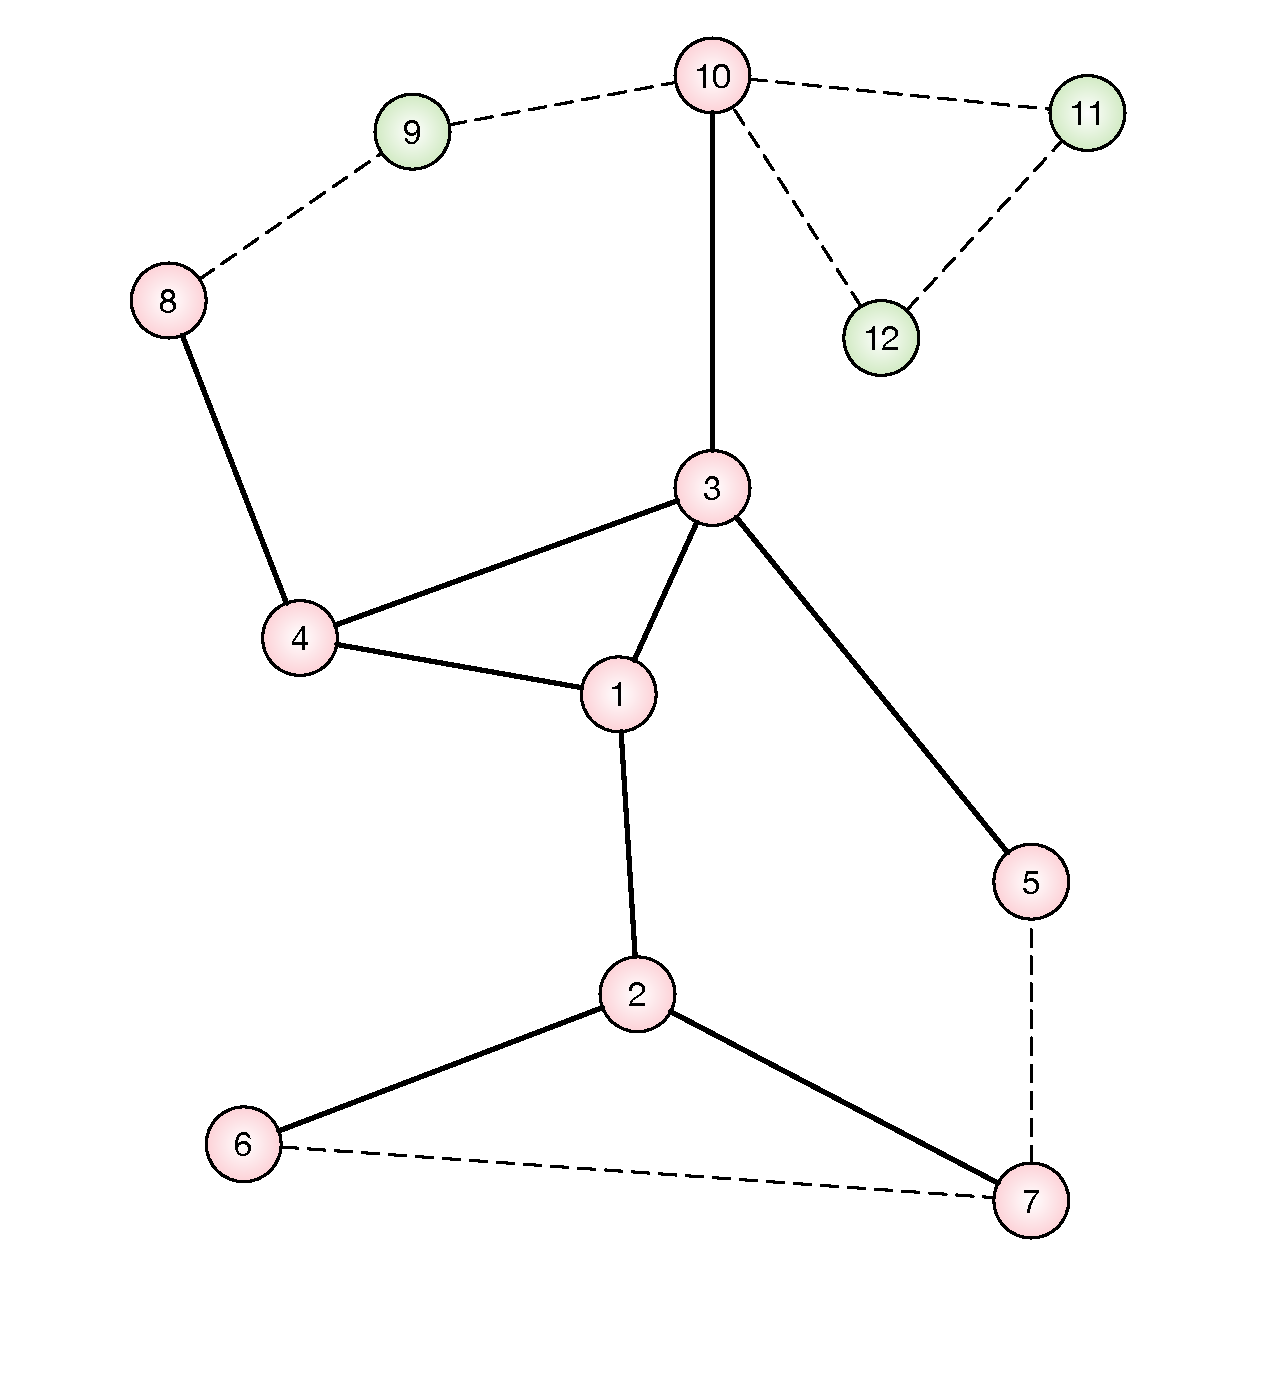
\includegraphics[width=.8\linewidth]{teixieraNetwork2014_proximityGraph.pdf}
  \caption{$H_T$}
  \label{fig:TeixierasNetworkH}
\end{subfigure}
\begin{subfigure}{.2\textwidth}
  \centering
  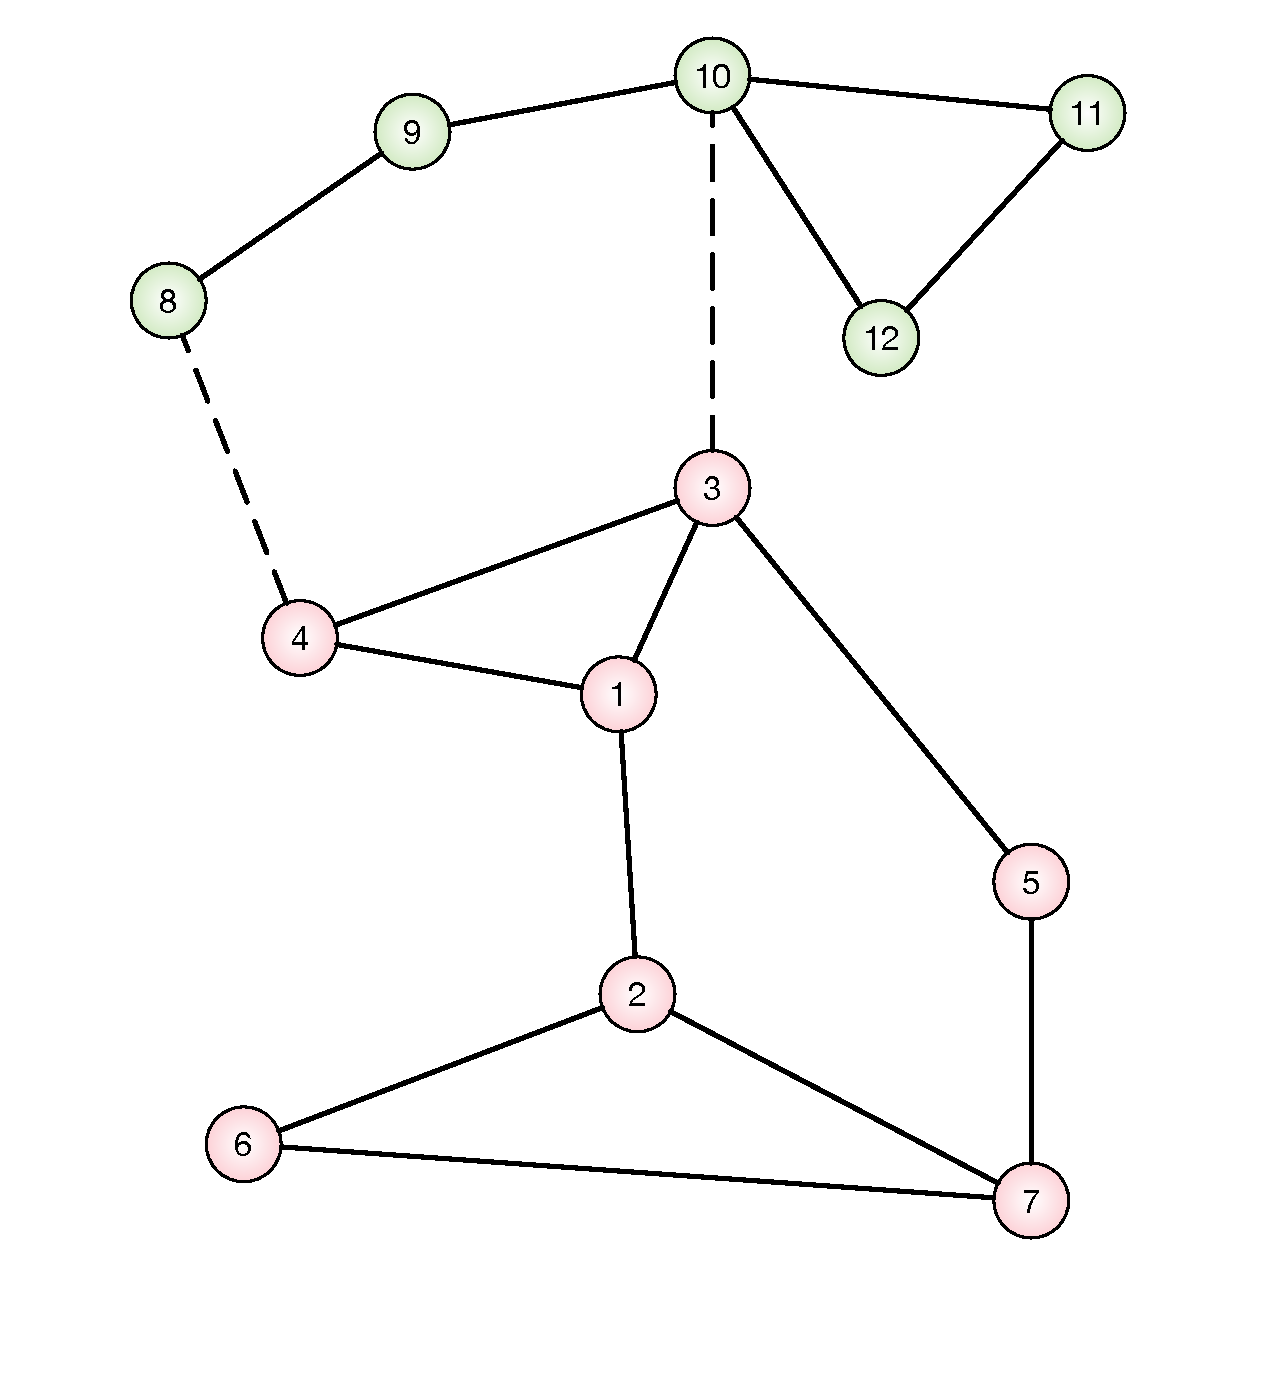
\includegraphics[width=.8\linewidth]{OurProposal.pdf}
  \caption{$H$}
  \label{fig:OurProposal}
\end{subfigure}
\caption{(A) The network used in an example from \cite{teixeira_distributed_2014}. (B) The network of monitoring agents proposed in \cite{teixeira_distributed_2014}, denoted here by $H_T$ (shown in red). (C) The network of monitoring agents $H$ (shown in red) ascertained through Algorithm \ref{alg:alg2}.}
\label{fig:fig}
\end{figure}
% \begin{figure}
%     \centering
%     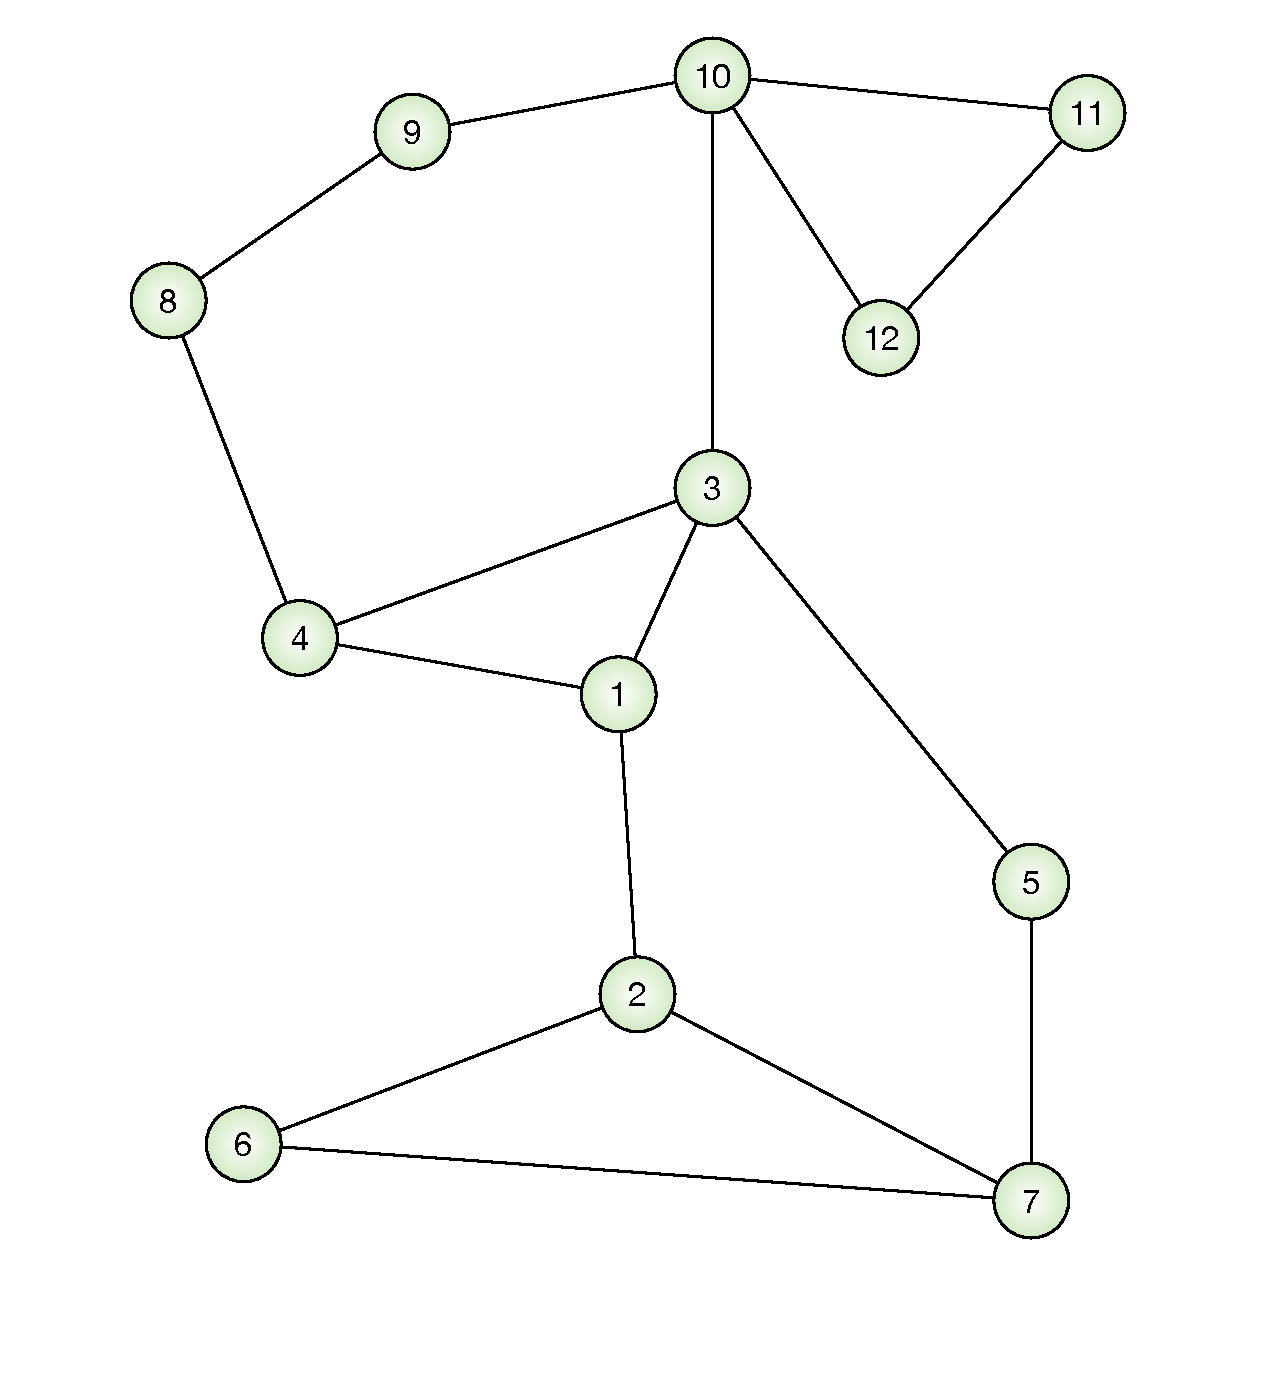
\includegraphics[scale=0.3]{teixieraNetwork2014.pdf}
%     \caption{The network used in an example from \cite{teixeira_distributed_2014}, denoted here by $G_T$.}
%     \label{fig:TeixierasNetworkCut}
% \end{figure}

% \begin{figure}
%     \centering
%     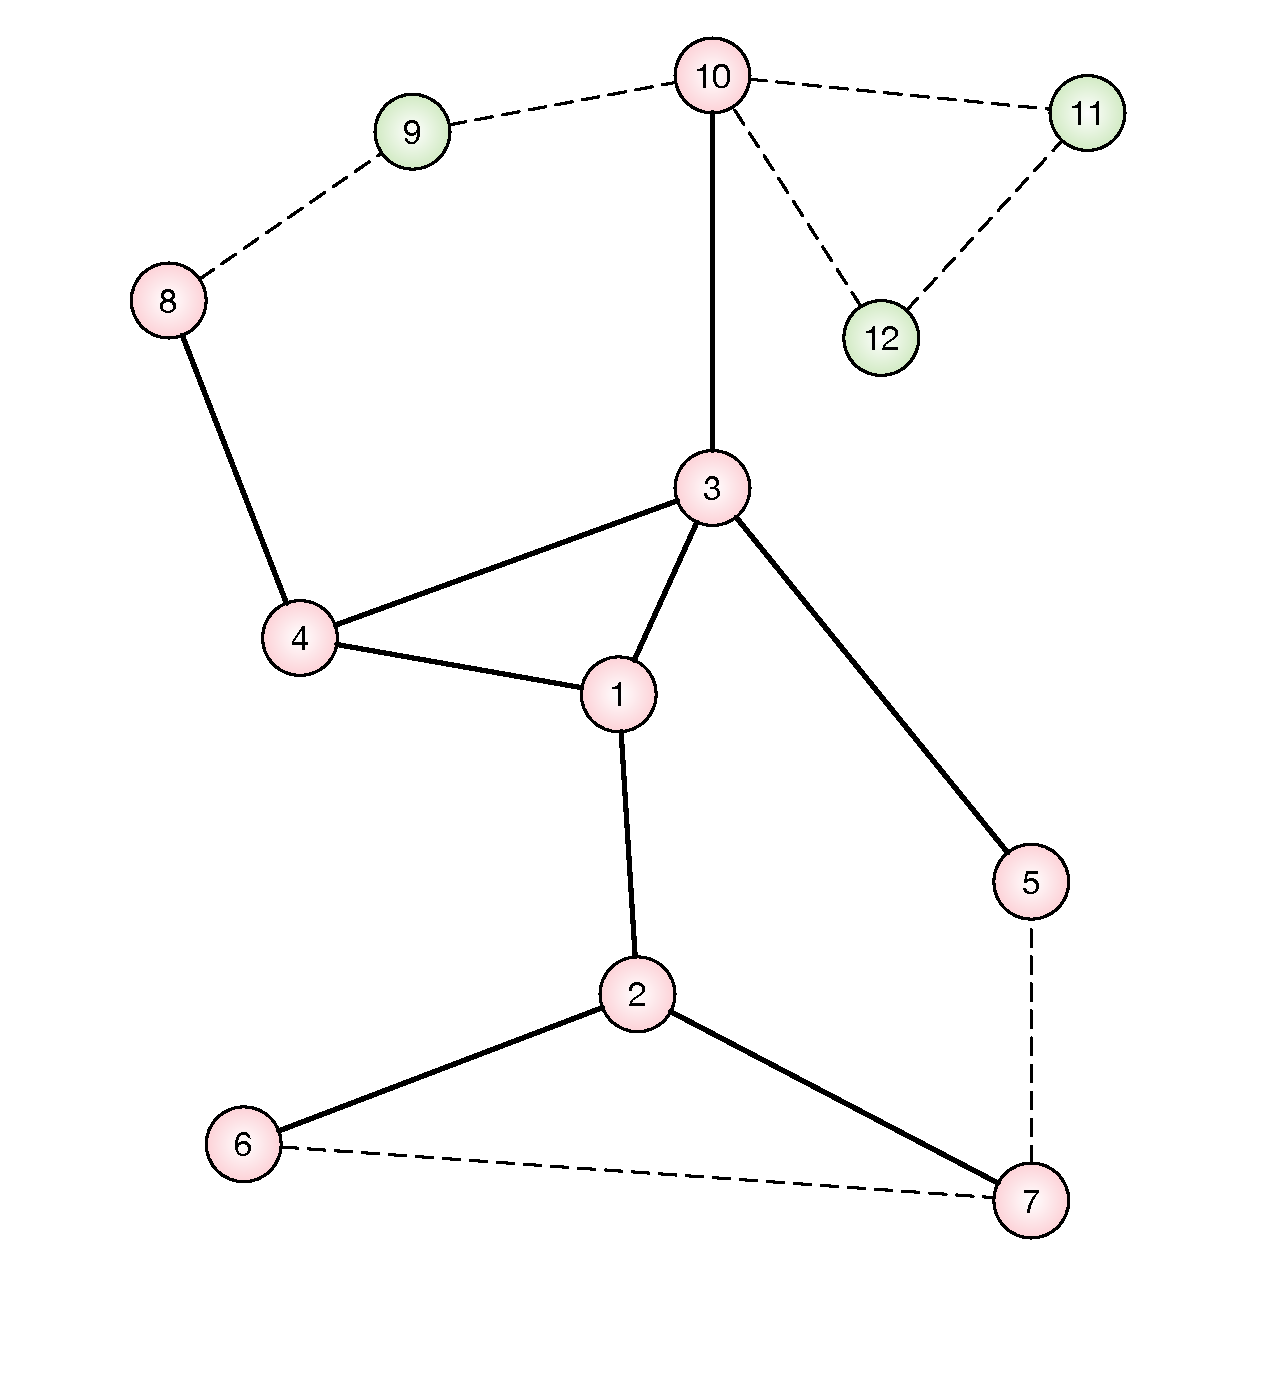
\includegraphics[scale=0.3]{teixieraNetwork2014_proximityGraph.pdf}
%     \caption{The network of monitoring agents proposed in \cite{teixeira_distributed_2014}, denoted here by $H_T$ (shown in red).}
%     \label{fig:TeixierasNetworkH}
% \end{figure}

% \begin{figure}
%     \centering
%     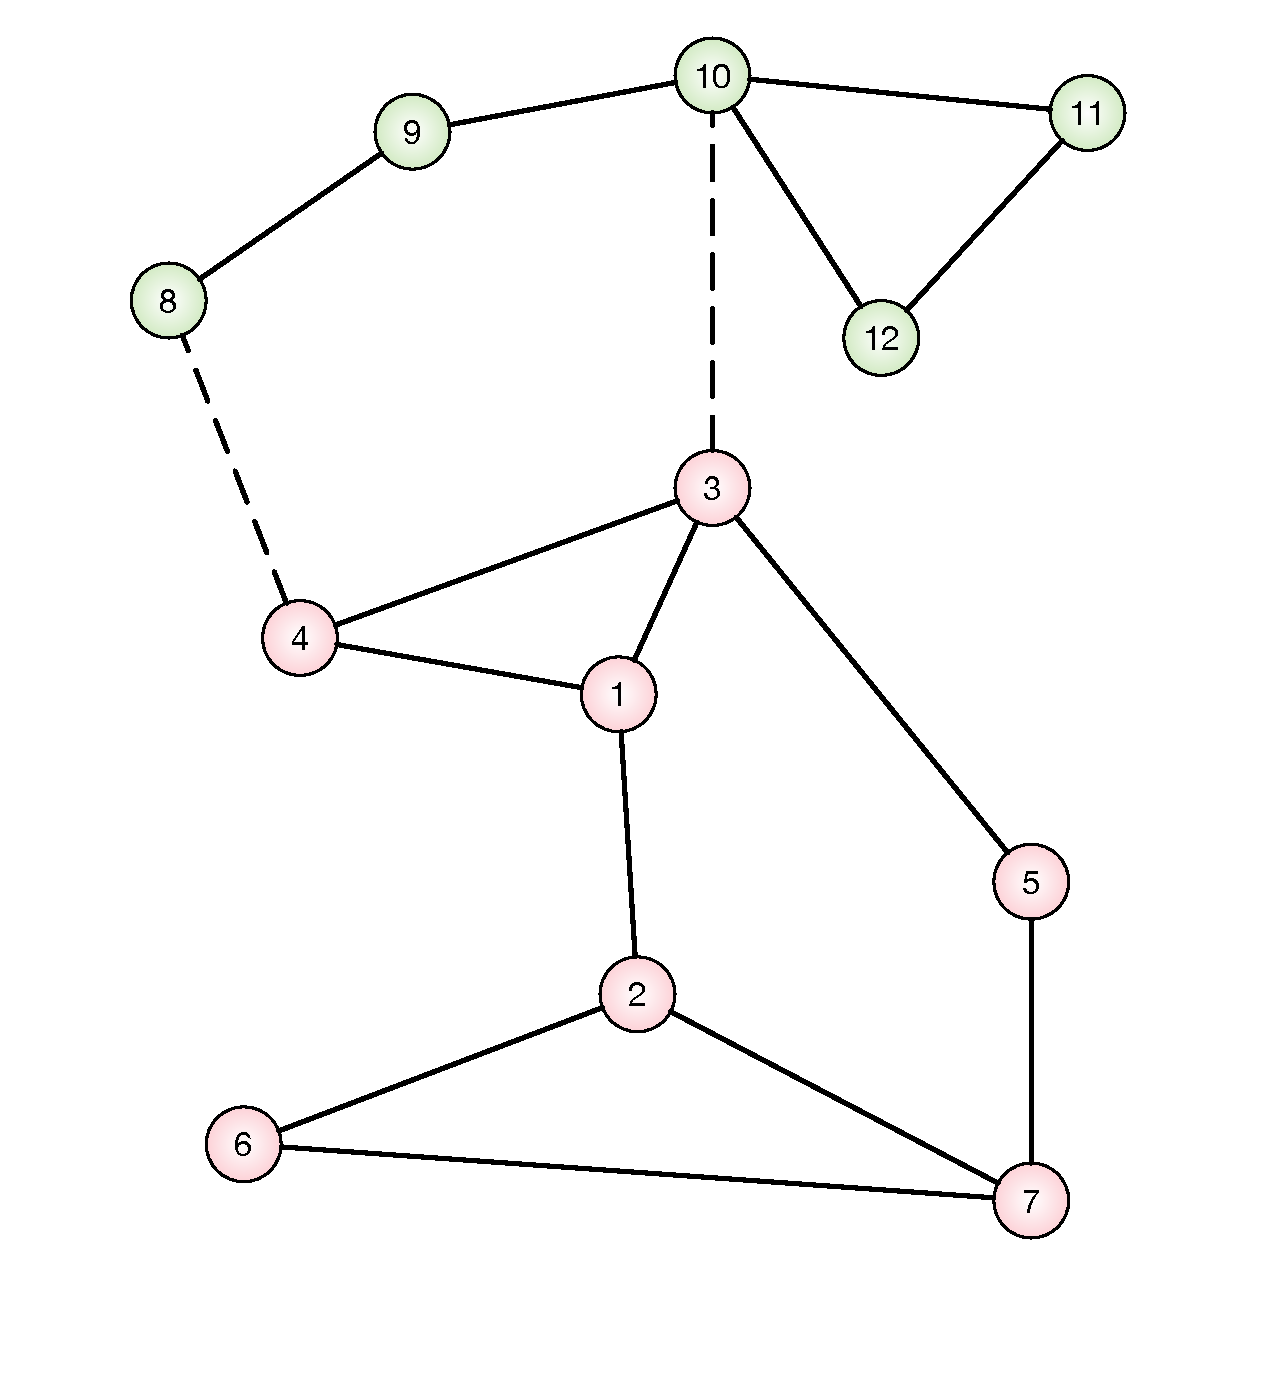
\includegraphics[scale=0.3]{OurProposal.pdf}
%     \caption{The network of monitoring agents $H$ (shown in red) ascertained through Algorithm \ref{alg:alg2}.}
%     \label{fig:OurProposal}
% \end{figure}

%where the authors proposed a solution based on the relaxation of the minimum total dominating set. Unfortunately, the minimum total dominating set does not ensure network robustness to attacks. 
% We consider the combinatorial expansion of the set $S$ as well as the network diameter and spectral expansion of an example given in \cite{teixeira_distributed_2014}, which is reproduced in Figure \ref{fig:TeixierasNetworkCut}A for convenience. These quantities are shown in Table \ref{tab:table1}.  In Figure \ref{fig:TeixierasNetwork}, the network considered in \cite{teixeira_distributed_2014} is reproduced. Using the approach suggested by the authors of \cite{teixeira_distributed_2014}, we have constructed the monitoring agent subgraph, $H$, shown in Figure \ref{fig:monitoringagents}. In Figure \ref{fig:TeixierasNetworkCut}, we illustrate how a sparse cut can disconnect a large fraction of the vertex set of $G$. In particular if an adversary was to sever or jam the links between monitoring agents \circled{4}-\circled{8} and \circled{3}-\circled{10}, then he/she can disconnect $60\%$ of the network by just removing $12\%$ of the network edges. The combinatorial expansion of the set $S:=\{1,2,3,4,5,6,7\}$ is 
% \begin{align*}
% h(S) = \frac{2}{7} = 0.29.
% \end{align*}
% and the spectral expansion is $\lambda_2^G = 0.125$ with a graph diameter of 5. Therefore, while the monitoring agents are able to sense the presence of intruders among all the agents in the network, the underlying topology that they form is vunerable to attacks from adversaries since the removal of only two edges results in a large fraction of the network being disconnected. 

% How shall the subgraph of the monitoring agents be chosen? A complete graph has too many edges and is not stable. What, if any, role does the graph diameter play? Let us consider the graph combinatorial expansion. Can the induced subgraph be chosen (or found) such that $h(G) \geq \epsilon$? This is the problem we are addressing. In other words, given $G$, is there $H$, an induced subgraph of $G$, such that $H$ belongs to a family of expander graphs? We formulate an optimization problem to address this. If $H$ exists and our optimization problem is feasible, then it returns the edge set for $H$. When our optimization problem fails to recover $H$, we provide explicit constructions, i.e. alterations to $G$ such that $H$ will have the property that if bla bla fraction of the edge set is removed then bla bla fraction of the vertices participate in the remaining connected component. 
% By Lemma \ref{lem:variational} the spectral expansion of $L$ can be written as:
% \begin{align*}
% \lambda_2 = \min_{\bof \in \R^n - \{0\}:\bof \perp \bof_1} \frac{\bof^T L_G \bof}{\bof^T\bof}
% \end{align*}
% It is easy to show that the quadratic form in the numerator is \cite{Merris1994}: 
%Let us expand the quantity in the numerator: 
% \begin{align}
% x^T Mx = \sum_{ij = 1}^n L_{ij} x_i x_j = \sum_{ij = 1}^n (D_{ij}-A_{ij}) x_i x_j,
% \end{align}
% and after distributing
% \begin{align} \label{eq:xmxExpand}
% \sum_{ij=1}^n (D_{ij} - A_{ij}) x_i x_j = \sum_{i = 1}^n D_{ii} x_i^2 - \sum_{ij \in \mathcal{E}(G)} 2x_i x_j.
% \end{align}
% The first term in (\ref{eq:xmxExpand}) is taken over the vertices of $G$ while the second term is taken over the edge set. It is possible to write both terms in terms of the edges of $G$, so we have:
% \begin{align}
% \bof^T L_G \bof = \sum_{ij \in \mathcal{E}(G)} (f_i - f_j)^2.
% \end{align}
% Throughout the paper we assume that $G_d$ is an undirected, unweighted, $d$-regular graph. We restrict our attention to unweighted graphs but all of our results naturally extend to weighted graphs. 
\begin{center}
\begin{table}
\caption{Graph invariants: Diameter, Connectivity and Spectral Expansion}
\begin{tabular}{|c|c|c|c|c|c|} 
	\hline
	Graph & $\cV$ & Diameter & Connectivity & Spectral Expansion & Approach\\
	\hline
    $G_T$ & 12 & 5 & 2 & $0.125$ & Proximity Method \cite{teixeira_distributed_2014} \\
	\hline
    $H_T$ & 9 & 4 & 1 & $0.184$ & Proximity Method \cite{teixeira_distributed_2014}\\
	\hline
    $H$ & 7 & 3 & 2 & $0.320$ & Algorithm \ref{alg:alg2}\\
    \hline
\end{tabular}\label{tab:table1}
\end{table}
\end{center}

% Finally, the network of monitoring agents is constructed according to Theorem \ref{thrm:margulisAgents}. Here the network of monitoring agents is not constrained by the edge set of the original graph, however we require that the vertex set be an even number. The network is shown in Figure \ref{fig:MargulisAgents}. The network diameter, connectivity and spectral expansion are tabulated in Table 1. 

% %-----------Conclusion------------
\section{Conclusion} \label{sec:sec5}
The algebraic and combinatorial conditions under which $H$ is maximally robust to attacks from external adversaries have been established. The algebraic conditions corresponding to the desirable combinatorial conditions that lead to resilient monitoring agent topology were stated in terms of a theorem and a corresponding spectral algorithm. The algorithm provided recovers the desired topology. Additionally, a result relating the third moment of $G$ to its spectral expansion was provided. The results were illustrated with an example. 
% \begin{figure}
% \begin{subfigure}{.35\textwidth}
%   \centering
%   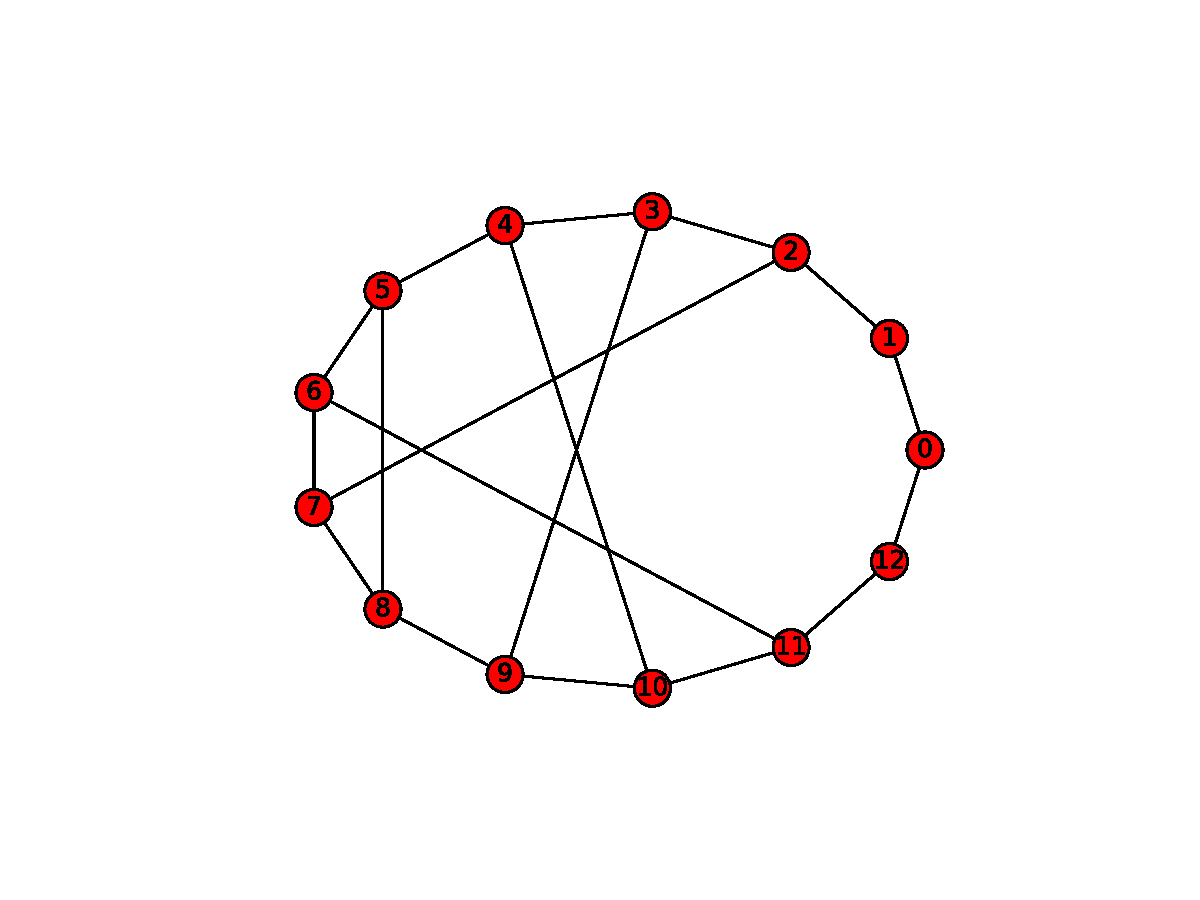
\includegraphics[width=.8\linewidth]{LBS.pdf}
%   \caption{$R_H$}
%   \label{fig:RamanujanAgents}
% \end{subfigure}%
% \begin{subfigure}{.35\textwidth}
%   \centering
%   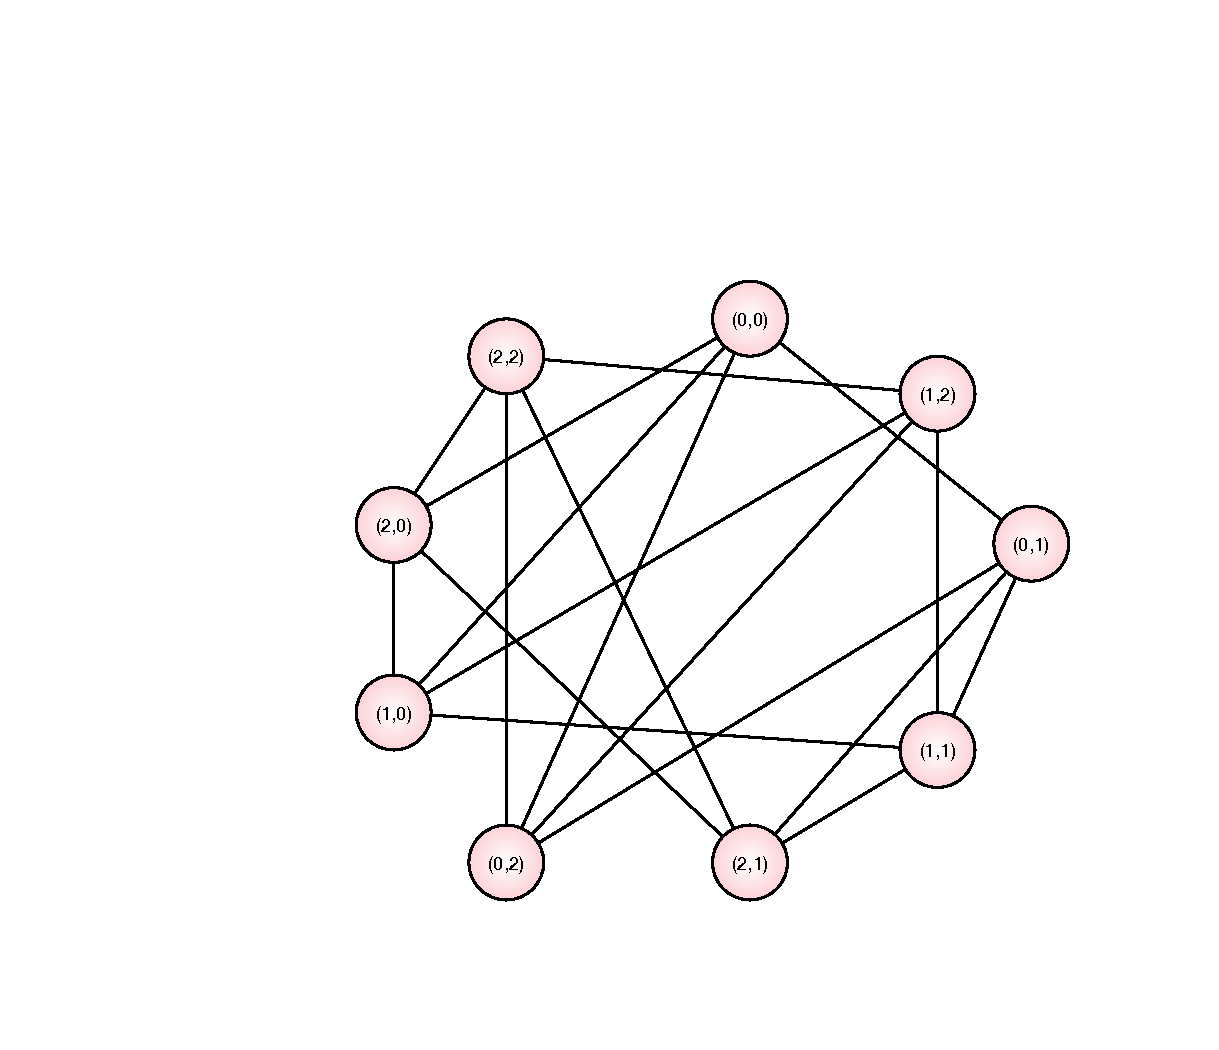
\includegraphics[width=.8\linewidth]{Margulis.pdf}
%   \caption{$M_H$}
%   \label{fig:MargulisAgents}
% \end{subfigure}
% \caption{(A) The Ramanujan network of monitoring agents, $R_H$. (B) The Margulis network of monitoring agents, $M_H$.}
% \label{fig:fig}
% \end{figure}
% %-----------BASICS-------------
% \section{Conclusion}

% \begin{figure}
%     \centering
%         \begin{minipage}{0.45\textwidth}
%             \centering
%             \includegraphics[scale=0.5]{lineGraph2Vertices.png} % first figure itself
%             \caption{Graph X}
%             \label{fig:graphX}
%         \end{minipage}\hfill
%         \begin{minipage}{0.45\textwidth}
%             \centering
%             \includegraphics[scale=0.5]{lineGraph3Vertices.png} % second figure itself
%             \caption{Graph Y}
%             \label{fig:graphY}
%         \end{minipage}
% \end{figure}

\bibliography{thesisBib}
\bibliographystyle{IEEEtran}
\end{document}
